\documentclass[pdftex,twocolumn,10pt,letterpaper]{extarticle}


% project related part
%\newcommand{\name}{\textsc{Janus}\xspace}
\newcommand{\name}{Giza\xspace}

\newcommand{\sm}[1]{\note{blue}{SM: #1}}
\newcommand{\ch}[1]{\note{blue}{CH: #1}}

%%% begin: packages added by Shuai
\usepackage{cleveref}
\usepackage{multirow}
\usepackage[symbol*]{footmisc}
\DefineFNsymbolsTM{myfnsymbols}{% def. from footmisc.sty "bringhurst" symbols
	\textasteriskcentered *
	\textdagger    \dagger
	\textdaggerdbl \ddagger
	\textsection   \mathsection
	\textbardbl    \|%
	\textparagraph \mathparagraph
}%
\setfnsymbol{myfnsymbols}
%%% packages added for appendix.
%boxruled, ruled, tworuled, plain
%vlined, lined, noline
%noend
\usepackage[linesnumbered,noresetcount,ruled,vlined]{algorithm2e}

% Compact itemize and enumerate.  Note that they use the same counters and
% symbols as the usual itemize and enumerate environments.
\def\compactify{\itemsep=0pt \topsep=0pt \partopsep=0pt \parsep=0pt}
\let\latexusecounter=\usecounter
\def\paritemize{%
        \setbox0\hbox{---}
        \list{---}{%
        \leftmargin\parindent
        \labelwidth\parindent
        \itemindent\z@
        \listparindent\parindent
        \parsep\z@
}%
}
\let\endparitemize\endlist
\newenvironment{CompactItemize}
  {\def\usecounter{\compactify\latexusecounter}
   \begin{itemize}}
  {\end{itemize}\let\usecounter=\latexusecounter}
\newenvironment{CompactEnumerate}
  {\def\usecounter{\compactify\latexusecounter}
   \begin{enumerate}}
  {\end{enumerate}\let\usecounter=\latexusecounter}


\def\codefontsmall{\fontsize{7}{8.75}\usefont{OT1}{phv}{m}{n}\selectfont}
\def\codefont{\usefont{OT1}{phv}{m}{n}\selectfont\footnotesize}

\newcommand{\tld}{\texttildelow}
\newcommand{\realnewpage}{\onecolumn\twocolumn}

\newcommand\KW[1]{\textbf{#1}} %keyword
\newcommand\CM[1]{\emph{#1}}   %comment
\newcommand\LA{$\gets$}  
\newcommand\INF{$\infty$}
\newcommand\GE{$\ge$}
\newcommand\NE{$\ne$}
\newcommand\TSCC{T\textsuperscript{SCC}}

\newcommand\IN{$\in$}
\newcommand\SIGMA{$\Sigma$}
\newcommand\CUPEQ{$\stackrel{\cup}{=}$}
\newcommand\OLDER {$\rightsquigarrow$}
\newcommand\DEFEQ{$\stackrel{\Delta}{=}$}
\newcommand\SUBI{\textsubscript{i}}
\newcommand\SUBA{\textsubscript{a}}
\newcommand\SUBB{\textsubscript{b}}
\newcommand\SUBONE{\textsubscript{1}}
\newcommand\SUBTWO{\textsubscript{2}}
\newcommand\SUPT{\textsuperscript{T}}
\newcommand\SUPP{\textsuperscript{p}}
\newcommand\SUPI{\textsuperscript{i}}
\newcommand\SUPD{\textsuperscript{d}}


\newcommand\LAR{$\leftarrow$}
\newcommand\RAR{$\rightarrow$}
\newcommand\UAR{$\Uparrow$}
\newcommand\RARONE{${\stackrel{1}{\rightarrow}}$}
\newcommand\RARTWO{${\stackrel{2}{\rightarrow}}$}
\newcommand\RARTHREE{${\stackrel{3}{\rightarrow}}$}
\newcommand\RARK{${\stackrel{k}{\rightarrow}}$}
\newcommand\RARI{${\stackrel{i}{\rightarrow}}$}
\newcommand\RARD{${\stackrel{d}{\rightarrow}}$}
\newcommand\IIE{${\stackrel{\mathfrak{ii}}{\mbox{---}}}$}


\newcommand\SRZT{the serialization graph}
\newcommand\SRZP{$\mathcal{S}^p$}
\newcommand\SRZ{serialization graph}
\newcommand\DEPT{$dep$}
\newcommand\DEPP{$\mathcal{D}^p$}
\newcommand\DEP{$\mathcal{D}$}
\newcommand\CHP{$\mathcal{C}$}
\newcommand\TRAR{${\leadsto}$}
%\newcommand\AFNRAR{${\looparrowright}$}
%\newcommand\AFNRAR{${\mathrlap{++}\rightarrow}$}

\newcommand\ORAR{${\mathrlap{o}\rightarrow}$}
\newcommand\NRAR{$\nrightarrow$}
\newcommand\TRARI{${\stackrel{i}{\leadsto}}$}
\newcommand\TRARD{${\stackrel{d}{\leadsto}}$}
\newcommand\TSRAR{${\mathrlap{*}\leadsto}$}
\newcommand\SRAR{${\mathrlap{*}\rightarrow}$}

%%% end: packages added by Shuai.



%%% Set these variables appropriately
%%%
%% Note:  Authors is hardcoded below, this line only used for the PDF info
\newcommand{\AUTHORS}{Paper \#xxx}
%\newcommand{\TITLE}{JANUS: Jesus! Another traNsaction and consensUS protocol}
%\newcommand{\TITLE}{Unifying Concurrency Control and Consensus for More Commits and Lower Latency}
\newcommand{\TITLE}{Project Giza: Replicating Erasure Coded Objects \\ across Global Data Centers}
\newcommand{\KEYWORDS}{Put your keywords here}
\newcommand{\CONFERENCE}{Somewhere}
\newcommand{\PAGENUMBERS}{yes}       % "yes" or "no"
\newcommand{\COLOR}{yes}
\newcommand{\showComments}{yes}
\newcommand{\comment}[1]{}
\newcommand{\onlyAbstract}{no}

%%%%%%%%%%%%%%%%%%%%%%%%%%%%%%%%%%%%%%%%%%%%%%%%%%%%%%%%%%%%%%%%%%%%%


%%%
%%%  Fonts
%%%
\usepackage[T1]{fontenc}
\usepackage[utf8]{inputenc}
\usepackage{newtxtext,newtxmath}                        % Times/Times-like math symbols
\usepackage{bm}
\usepackage{courier}
\usepackage[scaled=0.92]{helvet}


%%%
%%%  Page Setup
%%%
\special{papersize=8.5in,11in}
\setlength{\pdfpagewidth}{8.5in}
\setlength{\pdfpageheight}{11in}

\usepackage{ifthen}
\ifthenelse{\equal{\PAGENUMBERS}{yes}}{%
  \usepackage[nohead,
            left=1.0in,right=1.0in,top=1.0in,
            footskip=0.5in,bottom=1in,     % Room for page numbers
            columnsep=0.25in
            ]{geometry}
}{%
\usepackage[noheadfoot,left=1.0in,right=1.0in,top=1.0in,
            footskip=0.5in,bottom=1in,
            columnsep=0.25in
	    ]{geometry}
}

%%%
%%%  Captions
%%%
\usepackage[font=bf]{caption}
\usepackage{subcaption}
%\usepackage{subfig}
%%  Space between figure and caption (assuming caption
%%  is below figure)
%\usepackage[font=bf,aboveskip=0pt]{caption} % SPACE
%%  Space between caption and body text of document
%\addtolength{\textfloatsep}{-7pt} % SPACE

%%%
%%%  Section headings
%%%
\usepackage[compact]{titlesec}
%\titlespacing{\paragraph}{0pt}{*1}{*1}      % SPACE
%\titlespacing{\section}{0pt}{1pt}{1pt}      % SPACE
%\titlespacing{\subsection}{0pt}{2pt}{1pt}      % SPACE
%\usepackage[compact]{titlesec}              % SPACE
%\titleformat{\section}%                     % IEEE/ACM: caps + period
%  {\bf\large\uppercase}{\thesection.\quad}{0pt}{}

%%% fixing bug of section number missing
\usepackage{etoolbox}
\makeatletter
\patchcmd{\ttlh@hang}{\parindent\z@}{\parindent\z@\leavevmode}{}{}
\patchcmd{\ttlh@hang}{\noindent}{}{}{}
\makeatother
%%% end fixing

%%%
%%%  Lists
%%%
\usepackage{enumitem}
\setlist{itemsep=0pt,parsep=0pt}             % more compact lists

%%%
%%%  Header / Footer
%%%
\usepackage{fancyhdr}
\renewcommand{\headrulewidth}{0pt}

\ifthenelse{\equal{\PAGENUMBERS}{yes}}{%
  \pagestyle{plain}
}{%
  \pagestyle{empty}
}

%%%
%%%  Bibliography
%%%
\usepackage[numbers]{natbib}

%%%
%%%  Footnotes / Endnotes
%%%
\interfootnotelinepenalty=10000  % Split footnotes are annoying

% If you want endnodes, uncomment:
%\usepackage{endnotes}
%\usepackage{drafthead}
%\let\footnote=\endnote

%%%
%%%  Tables
%%%
\usepackage{booktabs}
\usepackage{color}
\usepackage{colortbl}
\usepackage{float}                           % Must appear before hyperref to
                                             % avoid weird PDF compile issues

%%%
%%%  PDF setup
%%%
\ifthenelse{\equal{\COLOR}{yes}}{%
  \usepackage[colorlinks]{hyperref}%         % for online version
}{%
  \usepackage[pdfborder={0 0 0}]{hyperref}%  % for paper (B&W) version
}
\usepackage{url}

\hypersetup{%
pdfauthor = {\AUTHORS},
pdftitle = {\TITLE},
pdfsubject = {\CONFERENCE},
pdfkeywords = {\KEYWORDS},
bookmarksopen = {true}
}

% Uncomment next line if your printer outputs black
% boxes instead of drop shadows; older PDF interpreters
% in printers can't handle those PDF 1.5 features
%\pdfminorversion=3
%\pdfobjcompresslevel=2


%%
%% Figure placeholder macros
%%

\definecolor{placeholderbg}{rgb}{0.85,0.85,0.85}
\newcommand{\placeholder}[1]{%
\fcolorbox{black}{placeholderbg}{\parbox[top][1.5in][t]{0.95\columnwidth}{#1}}}


%%%
%%%  Misc
%%%
\usepackage[pdftex]{graphicx}
\usepackage{soul}
% this allows \st and friends to work with citations
\soulregister\cite7
\soulregister\ref7
\soulregister\pageref7

%\setlength{\parindent}{2pt}
%\setlength{\parskip}{\baselineskip}

%\clubpenalty=10000  % Don't allow orphans
%\widowpenalty=10000 % Don't allow widows

%%%
%%%  To appear/appeared in text on title page
%%%
\usepackage[absolute]{textpos}
\newcommand{\ToAppear}{%
\begin{textblock*}{\textwidth}(0.95in,0.4in)
\begin{flushright}
    %\noindent{\fbox{\textsf{Under submission---please do not redistribute.}}}
    %  --OR--
    \noindent{\small To appear in \textit{Proceedings of the XYZ}\\
    \noindent{\small \textit{Conference (XYZ'08)}, City, State, Month 2008}}
    %  --OR--
    %\noindent{\small In \textit{Proceedings of the XYZ}\\
    %\noindent{\small \textit{Conference (XYZ'08)}, City, State, Month 2008}}
\end{flushright}
\end{textblock*}
}

%%%
%%%  Sample ACM Copyright Block
%%%
\newfloat{acmcr}{b}{acmcr}
\newcommand{\AcmCopyright}{%
\begin{acmcr}
\parbox[b]{20pc}{%
\footnotesize
Permission to make digital or hard copies of all or part of this work
for personal or classroom use is granted without fee provided that
copies are not made or distributed for profit or commercial advantage
and that copies bear this notice and the full citation on the first
page.  To copy otherwise, to republish, to post on servers or to
redistribute to lists, requires prior specific permission and/or a fee.

{\em Conference}, Month Date--Date, Year, Location\\
Copyright 200X ACM X-XXXXX-XX-X/XX/XX ...\$5.00}
\end{acmcr}}

%%%
%%%  Comments
%%%
\newcommand{\note}[2]{
    \ifthenelse{\equal{\showComments}{yes}}{\textcolor{#1}{#2}}{}
}

% Change these to your own initials as you like...
\newcommand{\dga}[1]{\note{blue}{Author1: #1}}
\newcommand{\mk}[1]{\note{red}{Author2: #1}}
\newcommand{\srini}[1]{\note{green}{Author3: #1}}

\date{}
\title{\vspace{-2ex} \textbf{\TITLE}}
\author{{\large \AUTHORS}}%\\
%{\em Affiliations}}

% This needs to be the last thing before \begin{document}
%\usepackage{microtype}  % SPACE

%%%%%%%%%%%%%%%%%%%%  START DOCUMENT  %%%%%%%%%%%%%%%%%%%%%%%%




%%%%%%%%%%% space savor
%%%%%%%%%%% space savor
%%%%%%%%%%% space savor
%%%%%%%%%%% space savor


%\usepackage{titling}
%\setlength{\droptitle}{-5em}   % This is your set screw
%\setlength\floatsep{10pt}
%\setlength\textfloatsep{10pt}
%\setlength\intextsep{10pt}
%\setlength{\abovecaptionskip}{2pt}
%\setlength{\belowcaptionskip}{0pt}


\begin{document}

\maketitle

%\AcmCopyright
%\ToAppear

\begin{abstract}

%Competition and scale are the two main forces driving cloud storage providers to apply erasure coding for better durability and lower cost. Today, all the major cloud storage providers encode customer data within individual data centers. The same economics forces are now pushing cross-DC erasure coding as the new forefront. We argue that the right time has finally arrived.

All major cloud storage providers have been driven by competition and scale to erasure code customer data within individual data centers. Now, the same economic force is pushing cross-DC erasure coding as the new forefront. The right time has arrived.

This paper presents the design, implementation and evaluation of Giza - a strongly consistent, versioned object store that encodes and store objects across global data centers. Giza separates each {\em get} and {\em put} operation into data and meta-data path, each of which is built on top of existing cloud storage systems. 
This architecture choice leads to simplified development, deployment and operation. Giza implements the Paxos consensus algorithms to achieve strong consistency. We address unique challenges of implementing Paxos with restricted cloud storage APIs. Giza is jointly optimized on both the data and metadata path. As a result, Giza is fast in normal operation for our target workloads.

Giza is deployed to \deployment and our evaluation demonstrates its effectiveness. We compare Giza to CockroachDB, which is considered an open source implementation of Spanner. The comparison shows that Giza achieves much lower latency than naively adopting a globally consistent storage system.

\end{abstract}

%%% Local Variables:
%%% mode: latex
%%% TeX-master: "main"
%%% End:
%\name{} unifies concurrency control and consensus by explicitly tracking the
%dependencies among transactions at server replicas involved in the
%transactions.  It collects and aggregates the dependency graph in one or two
%round-trips during transaction commit.  Doing so allows servers to
%deterministically break any cycles detected in the dependency graph by
%re-ordering operations whose execution is deferred to commit time.  

\ifthenelse{\equal{\onlyAbstract}{no}}{%
\section{Introduction}

\subsection{Cross-DC Erasure Coding: Why Now?}

As the entire IT industry is rapidly moving to the cloud, more and more data
centers are being built all over the globe. The event that one of the data
centers will fail catastrophically becomes inevitable over time. In other words,
this is no longer a matter of ``if'', but rather ``when''. 
%{\em Designing for disasters}~\cite{keeton04designing} becomes essential and
Data stored in the
cloud have to be protected against catastrophic data center failure.

There have been a long line of prior work~\cite{oceanstore:asplos00, pond:fast03,
weatherspoon2005long, hail:ccs09, racs:socc10, hu12nccloud} arguing for storing data
in erasure coded form, as opposed to replication, across geo-graphically
distributed data centers. Compared to geo-replication, cross-DC erasure coding
tolerates data center failure and ensures durability, while significantly
reduces storage cost. The same economic force that has driven cloud providers to
erasure code data within individual data centers naturally extends to the
cross-DC scenario.

Nevertheless, none of the cloud providers today offer options to erasure code
customer data across data centers. This is largely due to the prohibitive cost
of cross-DC network traffic. The reduction in storage cost comes to balance the
additional cost of inflated cross-DC network traffic, for both read/write during
normal operation and access/rebuild in the event of data center failure, as
discussed in detail in Section~\ref{sec:motivation}. Since the total cost of
storing customer data needs to cover both the storage and the cross-DC network
traffic, cross-DC erasure coding has not seen wide deployment yet.

%\begin{table}[thp]
%\centering
%\small
%\begin{tabular}{|l|c|c|}
%\hline
%TransAtlantic Cable             & FLAG Atlantic 1~\cite{bib:FA-1}   & MAREA~\cite{bib:MAREA1, bib:MAREA2}
%\\ \hline \hline
%Ready For Service               & 2001                              & 2017
%\\ \hline
%Cost (Billion)                  & 1.1                               & undisclosed
%\\ \hline
%Capacity                        & 10 Gbps                           & 160 Tbps
%\\ \hline \hline
%\end{tabular}
%\caption{Cross-DC bandwidth cost reducing by orders of magnitude.}
%\label{tab:mears}
%\end{table}
Fortunately, technological breakthroughs in wide area networking have dramatically reduced cross-DC bandwidth cost.
There are two key driving forces. 1) The erbium-doped fiber
amplifiers~\cite{mears1986low} make it practical to amplify a huge spectrum of
optical signal directly, without the need to convert to electrical signal.
2) Dense Wave Division Multiplexing (DWDM) is in turn enabled by the fiber
amplifiers, which can send 10+ terabits per second over single fiber~\cite{zhu2011112}.
Most recently, Facebook and Microsoft have teamed up to build $MAREA$, a new
fiber optic cable under the Atlantic Ocean that uses eight pairs of fiber optic
strands and will come online in 2017 with 160 Tbps capacity~\cite{bib:MAREA1, bib:MAREA2}.
In comparison, a transatlantic cable dated back in 2001 cost 1.1 billion dollars,
but had a mere capacity of 10 Gbps~\cite{bib:FA-1}.
Hence, MAREA represents over 10,000$\times$ bandwidth increase in less than two decades.
%While the cost of MAREA remains undisclosed, it suffices
%to say that cross-DC bandwidth cost has reduced by several orders of magnitude.
The significant cost reduction in cross-DC bandwidth is now
making cross-DC erasure coding economically attractive.

\comment{bib:MAREA1, http://www.wsj.com/articles/facebook-and-microsoft-to-build-fiber-optic-cable-across-atlantic-1464298853}
\comment{bib:MAREA2, http://www.usatoday.com/story/experience/2016/05/26/microsoft-facebook-undersea-cable-google-marea-amazon/84984882/}
\comment{bib:FA-1, https://en.wikipedia.org/wiki/Fiber-Optic_Link_Around_the_Globe}

\begin{figure}[tp]
\centering
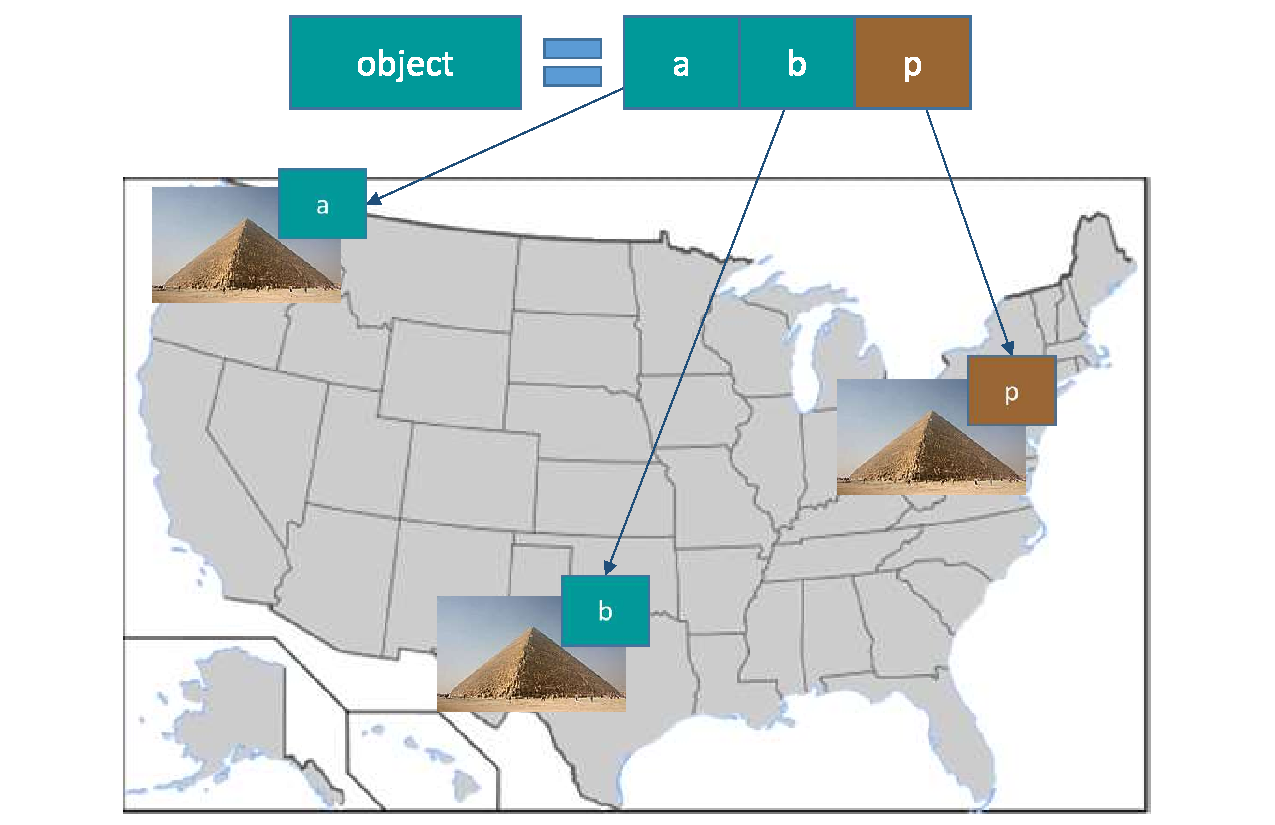
\includegraphics[width=0.4\textwidth]{images/giza_example_crop_fit}
\caption{Storing Object in Giza}
\label{fig:giza_example}
\end{figure}

\subsection{Giza Overview}

Giza exploits the reduction in cross-DC bandwidth cost
and leverages erasure coding to optimize the total cost of storing customer data in the cloud.
It offers an externally strong consistent (linearizable~\cite{herlihy90linearizability}),
versioned object store that erasure codes objects across global data centers.
Customers access Giza by creating Giza storage accounts. For each storage
account, the customers have the flexibility to choose the set of data centers
where their data are striped across. In addition, they can specify erasure coding scheme.
Giza employs classic $n = k + m$ Reed-Solomon coding, which generates $m$ parity fragments from $k$ data fragments.
All coded fragments are stored respectively in $n$ different DCs,
so as to tolerate up to $m$ arbitrary DC failures.
%By allowing the customers to choose the set of data centers and specify the erasure coding scheme, Giza gives the customers complete control of storage overhead and durability.
The customers access Giza with straightforward {\em put}, {\em get} and {\em delete} interface. In addition, Giza supports versioning, where new {\em put} does not overwrite existing data, but rather creates a new version of the same data. The old version remains available until it is explicitly deleted.

Giza operates on top of existing cloud storage systems that offers reliable and redudant local data storage. It stores data
objects in cloud blob storage and the metadata of the objects in cloud table
storage. Figure~\ref{fig:giza_example} illustrates an exemplary flow of storing
an object in Giza with 2 + 1 erasure coding.
%Giza operates a number of {\em stateless} Giza nodes in every data center. Say a customer uses a Giza client (command line, library, or REST interface) to store a 4MB data object. The Giza client routes the {\em put} request to one of the Giza nodes in the data center closest to the customer.
Giza divides the object into two data fragments ($a$ and $b$) and encodes them to a parity fragment $p$.
The fragments are stored respectively in the blob storage in three data centers. The metadata, consisting of the pointers to the
blobs, as well as versioning information, is replicated in the table storage across the
same data centers.

\subsection{Challenges and Contributions}

Giza targets cloud drive services which store predominantly large objects, such as
Dropbox, Google Drive, and Microsoft OneDrive, etc.
The design is motivated by the workload of such services observed in Section~\ref{sec:motivation}
and summarized here:
1) large storage space consumption,
2) cold data, where only a tiny percentage of objects are accessed
beyond a short period after creation,
3) objects may be updated over time, but concurrent updates of the same
object are rare (albeit possible).

Given the target workload, Giza optimizes for the common case, where there is
a single writer and multiple readers. Giza strives to {\em make the common case
fast}. In fact, the most optimized version of Giza achieves optimal latency,
which is a single cross-DC round trip for both {\em put} and {\em get}.

On the other hand, Giza handles the rare case properly,
and provides strong consistency when concurrent updates to the same object {\em do} occur.
%For instance, Giza tolerates data center failure. In the
%event of a data center being temporarily unavailable (or simply slow), the
%customers are able to continue to read and write data objects without much
%impact. The unavailable (or slow) data center may miss updates, which could
%potentially lead to conflict when they receive new updates again.
%For instance,
%the retry of a {\em put} could be processed by a different server (or even DC)
%and results in conflict with the previously unfinished {\em put}.
%Even though concurrency is rare,
%it is crucial for Giza to {\em guarantee the rare case correct}.
% Indeed, Giza provides external consistency.

Giza operates on top of existing cloud storage systems. 
The blob and table storage within individual data centers operate independently.
Hence, while strongly consistent individually, the collection of the blob and
table storage across multiple data centers do not readily offer the desired
external strong consistency. The key technical challenge Giza addresses is how to achieve
optimal latency with single {\em put}, while at the same time provide
strong consistency under concurrency, over the collection of individual blob and
table storage across multiple data centers.

Towards this end, the paper makes the following contributions:
\begin{itemize}
    \item We have designed and implemented Giza, a strongly consistent,
      versioned object store that erasure codes objects across globally
      distributed data centers.
    \item Giza is fast in the common case: when there is no concurrency, Giza
      completes within a single cross-DC round trip, which is optimal given the
      requirement to tolerate data center failure.
    \item Giza provides strong consistency when accessed concurrently, even with data center
      failure.
    \item Giza employs well-known distributed algorithms, such as Paxos~\cite{lamport01paxos}
      and Fast Paxos~\cite{lamport05fast}, in a novel way so that it operates on top of existing cloud storage
      systems.
    \item Giza is deployed in \deployment. Experimental results demonstrate
      that Giza achieves all our design goals. In particular, it is worth
      pointing out that Giza achieves much lower latency than naively adopting a
      globally consistent storage system, like CockroachDB (widely considered as open source
      implementation of Google's Spanner).
\end{itemize}

\section{The Case for Giza}
\label{sec:motivation}

This section presents the characteristics of a large-scale cloud drive service with hundreds of millions of users. These characteristics motivate the design choices of Giza.
%The section is concluded with a discussion of an alternative approach.

\subsection{Cloud Drive Characteristics}

\begin{figure}[tp]
%\centering
\hspace{-3em}
\begin{subfigure}{.3\textwidth}
  \centering
  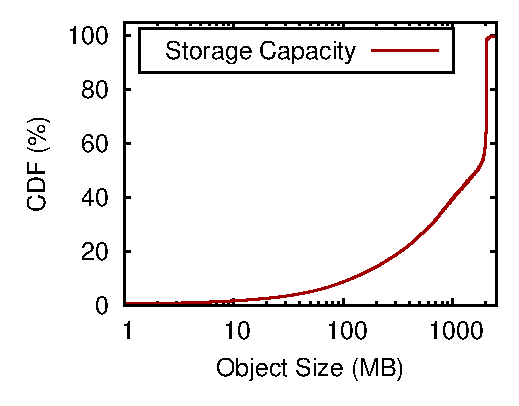
\includegraphics[width=\linewidth]{data/object_size-storage_capacity}
  \caption{}
  \label{fig:object_size-storage_capacity}
\end{subfigure}%
%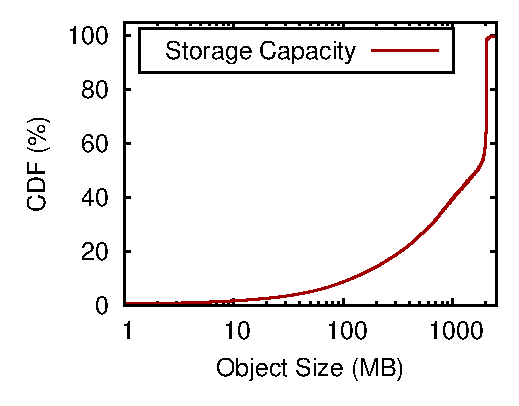
\includegraphics[width=0.5\textwidth]{data/object_size-storage_capacity}
%\hspace{-2em}
\begin{subfigure}{.3\textwidth}
  \centering
  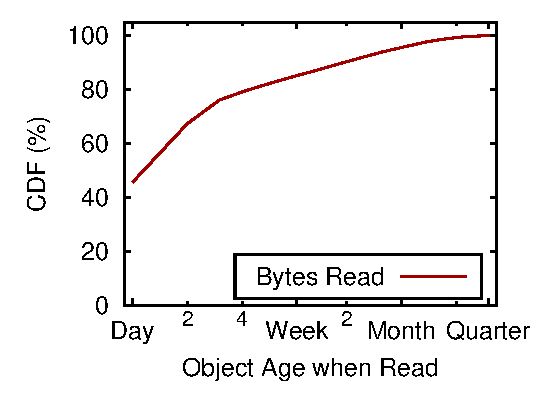
\includegraphics[width=\linewidth]{data/write_read_gap-bytes_read}
  \caption{}
  \label{fig:write_read_gap-bytes_read}
\end{subfigure}%
\caption{Cloud Drive Characteristics}
\label{fig:case_for_giza}
\end{figure}

{\bf Methodology:} The data presented in this section is derived from a three-month trace of a tier-1 cloud drive service. The cloud drive serves hundreds of millions of users and stores their objects, including documents, photos, music, videos, configuration files and more. The trace includes {\em all} reads, writes and updates to {\em all} objects between January 1 and March 31, 2016. We observe the following:

{\bf Large Objects Dominate:} The size of the objects varies significantly, ranging from Kilobytes to tens of Gigabytes. While the number of small objects vastly exceeds that of large objects, the storage capacity occupied by the small objects turns out to be small. Figure~\ref{fig:object_size-storage_capacity} presents the cumulative distribution of storage capacity consumption in terms of object size. We observe that less than $0.9\%$ of the total storage capacity is occupied by objects smaller than 4MB. This suggests that, to optimize storage cost, it is sufficient for Giza to focus on objects of 4MB and larger~\footnote{Objects of tens of Gigabytes are divided into 4MB chunks before storing in cloud storage back-end.}. Objects smaller than 4MB can simply use the existing geo-replicated storage system. This design choice reduces the overhead associated with erasure coding of small objects (including meta-data for the smaller object). As a result, all following analysis filter out objects smaller than 4MB.

{\bf Object Temperature Drops Fast:} A common usage scenario of cloud drive is sharing. Objects stored in the cloud drive are often shared across multiple devices, as well as among multiple users. Therefore, it is typical to observe reads soon after the objects are created. To this end, Figure~\ref{fig:write_read_gap-bytes_read} presents the cumulative distribution of bytes read in terms of object age when the reads occur~\footnote{The analysis focuses on all the objects created during the three-month period. Hence, the object age is capped at three months.}. It is worth pointing out that $47\%$ of the bytes read occurred in the same day of object creation, $87\%$ occurred within the same week, and merely less $2\%$ occurred beyond one month. This suggests that the temperature of the objects drops at a fast space. Moreover, caching the objects for a short period of time can satisfy most of the reads (more below).

\begin{table}[h]
\footnotesize
\centering
\begin{tabular}{|c||c|c|}
\hline \hline
total reads (B) / writes (B) 	& \multicolumn{2}{c|}{2.3$\times$}
\\ \hline \hline
%\multirow{4}{*}{cross-DC reads / writes \newline in Giza}
	& no caching		& 1.15$\times$
\\ \cline{2-3}
cross-DC reads / writes
	& caching (day)		& 0.61$\times$ 
\\ \cline{2-3}
with Giza
	& caching (week)	& 0.18$\times$ 
\\ \cline{2-3}
	& caching (month)	& 0.05$\times$ 
\\ \hline \hline
\end{tabular}
%\caption{Giza with Caching in Local DC.}
\label{tab:caching}
\end{table}
{\bf Writes Dominate with Caching:} The above table presents the effectiveness of caching. The ratio between the total amount of bytes reads to writes is 2.3$\times$. 
%This implies that on average each object is read 2.3 times. 
As illustrated in Section~\ref{sec:alternative}, Giza incurs 1x and 0.5x cross-DC network traffic in writes and reads, respectively. Hence, the ratio between cross-DC traffic due to reads and writes is $1.15\times$. Given the temperature analysis, it is most effective for Giza to additionally cache  objects for a short period of time within one single DC. Serving reads from the caching DC dramatically reduces the cross-DC traffic due to reads. Indeed, when objects are cached for one day, the cross-DC traffic attribute to reads vs writes reduces to 0.61$\times$. When objects are cached for one month, the ratio reduces to negligible 0.05$\times$, where the cross-DC traffic is completely dominated by writes.

\begin{table}[h]
\footnotesize
\centering
\begin{tabular}{c||c|c|c}
\# of Versions 	& 	1				& 2					& $\ge 3$
\\ \hline
Percentage			& $57.96\%$	& $40.88\%$	& $1.16\%$
\end{tabular}
\label{tab:version}
\end{table}
{\bf Concurrency is Rare, but Versioning is Required:} The above table presents how often objects are updated and require versioning support. We observe that $57.96\%$ of the objects are written once and never updated during the three-month period. For the remaining, $40.88\%$ of the objects are updated exactly once and merely $1.16\%$ are updated more than twice. This suggests that concurrent updates of objects are rare in Giza (albeit possible). Hence, Giza focuses and optimizes for single writer, while at the same time supports versioning. 

%\subsection{Giza: Flexible Cross-DC erasure coding }
%
%Erasure coding across geo-graphically distributed data centers is a most effective approach to reduce storage cost while achieving the fault tolerance goal of being able to survive data center failure. As Facebook's F4 system~\ref{bib:F4} has demonstrated, replacing geo-replication with cross-DC erasure coding can effectively reduce storage overhead from 3.6x to 2.1x, achieving huge savings for Facebook's 65PB of warm storage. While a fixed 2 + 1 solution works very well for Facebook's special workload, the public cloud storage desires much more flexibility. Different customers have different desirable operating points in terms of cost, durability and latency trade-off and are willing to accept different pricing for individual needs. 
%
%Giza provide completes flexibility to the customers. When a storage account is created, the customers may specify how much fault tolerance is desired at the storage account level. In addition, the customers had additional flexibility to specify which data centers are involved, so that they could constraint all the data to be in the  United States per data sovereignty requirement and regulation, or they could choose to disperse the erasure coded data across multiple continents, so that no single country could gain access to the complete data. 

%\begin{table*}[tp]
%\centering
%\begin{tabular}{|l||c||c|c|c|c||c|c|}
%\hline
				%& Geo-Replication    	& \multicolumn{4}{c||}{Giza (standard durability)}		& \multicolumn{2}{c|}{Giza (enhanced durability)}
%\\ \hline \hline
%Number of DCs 				& 2										& 3 & 4 & 5 & 6									& 5 & 6
%\\ \hline
%Erasure coding scheme & replication					& 2 + 1 & 3 + 1 & 4 + 1 & 5 + 1	& 3 + 2 & 4 + 2
%\\ \hline \hline
%Storage overhead			& 2.6x								& 1.9x & 1.7x & 1.6x & 1.5x			& 2.1x & 1.9x
%\\ \hline
%Reduction							& -										& 27\% & 35\% & 38\% & 42\%			& 19\% & 27\%
%\\ \hline \hline
%WAN traffic (put)			& 1x									& 1x & 1x & 1x & 1x 						& 1.33x & 1.25x
%\\ \hline
%WAN traffic (get)			& 0										& 0.5x & 0.67x & 0.75x & 0.8x		& 0.67x & 0.75x
%\\ \hline
%DC rebuild 						& 1x									& 2x & 3x & 4x & 5x 						& 3x & 4x
%\\ \hline \hline
%\end{tabular}
%\caption{Trade-off of storage, bandwidth and durability.}
%\label{tab:cost_benefit}
%\end{table*}

\begin{table}[tp]
\centering
\footnotesize
\begin{tabular}{|l||c||c|c|c|}
\hline
											& Geo-Rep.						& \multicolumn{3}{c|}{Giza}
\\ \hline \hline
\# of DCs 						& 2										& 3 		& 5 		& 7
\\ \hline
Erasure coding 				& -										& 2 + 1	& 4 + 1	& 6 + 1
\\ \hline \hline
Storage overhead			& 2.6									& 1.9 	& 1.6 	& 1.5
\\ \hline
{\bf Cost savings}		& -										& {\bf 27\%} 	& {\bf 38\%} 	& {\bf 42\%}
\\ \hline \hline
cross-DC traffic (put)& 1x									& 1x 		& 1x 		& 1x
\\ \hline
cross-DC traffic (get)& 0										& 0.5x 	& 0.75x & 0.83x
\\ \hline
DC rebuild 						& 1x									& 2x 		& 4x 		& 6x
\\ \hline \hline
\end{tabular}
\caption{Giza Trade-offs}
\label{tab:cost_benefit}
\end{table}


\subsection{Giza Trade-offs}
\label{sec:alternative}

Compared to geo-replication, Giza offers more flexible trade-offs in terms of storage cost and cross-DC network traffic,
as summarized in Table~\ref{tab:cost_benefit}.
% summarizes the costs and benefits of Giza at various operating points.

{\bf Storage Cost:}
To tolerate single data center failure, geo-replication incurs the storage overhead of $2\times1.3$ = 2.6 (with single DC storage overhead at 1.3).
With $k+1$ erasure coding, where $k$ ranges from 2 to 6, Giza reduces the storage overhead to between 1.9 and 1.5, increasing cost savings from 27% to 42%.
The storage cost savings come with inflated cross-DC traffic, which is examined next.

{\bf Cross-DC Traffic:} For writes, Giza does {\em not} incur more cross-DC traffic than geo-replication. Objects are uploaded to any DC and processed by Giza in the DC. With $k+1$ erasure coding, the objects are divided into $k$ data fragments, where one fragment is stored in the DC locally and the rest $k$ fragments are stored in remote DCs. Hence, the ratio between cross-DC traffic and object size is $k/k = 1$, same as geo-replication.
For reads, however, Giza incurs additional cross-DC traffic. $k$ fragments are required to serve reads, where one is from the DC locally and the rest $k-1$ from remote DCs. Hence, the ratio between cross-DC traffic and object size is $(k-1)/k$, which increases with $k$. In comparison, geo-replication serves reads entirely from the DC locally and incurs no cross-DC traffic at all.
Upon data center failure, data originally stored at the failed DC needs to be rebuilt at a new DC. Geo-replication simply replicates every object and thus incurs 1x of cross-DC traffic. In contrast, Giza relies on erasure decoding to reconstruct missing fragments, each incurring $k$ times cross-DC traffic.

{\bf Alternative Approach:} Giza stripes individual objects across multiple DCs. This design leads to cross-DC traffic when serving reads. A possible alternative is to first aggregate objects into large logical volumes (say 100GB) and then erasure code different volumes across multiple DCs to generate parity volumes. Since every object is stored in its entirety in one of the DCs, cross-DC traffic is avoided during reads.

This design works great when objects are never deleted~\cite{f4:osdi14}. However, Giza must support deletion. Deleting objects from logical volumes (and canceling them from corresponding parity volumes) would result in complex bookkeeping and garbage collection, and greatly increases engineering complexity. In comparison, the design of Giza is much simpler, specially when (with caching enabled) reads only consume a small percentage of cross-DC traffic compared to writes. 

%%% Local Variables:
%%% mode: latex
%%% TeX-master: "main"
%%% End:

%% \section{Overview}

%% [TODO put this to a separate file and come with a plan]

%% [Shall we put the assumptions/setup here?]

%% [Shall we put the interface here?]

%% [Give a table, summarize the interface]

%% % \subsection{Interface and Assumptions}
%%                                 % Giza is an erasure coding scheme for key/value stores and provide two operations: Put(Key, Value) and Get(Key), where Key and Value are arbitrary strings. Get(Key) returns the value of the latest Put for that key. (Add assumptions here + what giza is good for: Giza provides fault tolerance for non byzantine failures in an asynchronous network)


%% % operations  semantics
%% % put         
%% % get 
%% % get_stale

%% \subsection{State Machine Replication and Paxos}

%% \subsection{Erasure coding}

\section{Design}

This section presents the design of {\name}, including the overall architecture,
the data model, and the protocols for the {\em put}, {\em get} and {\em delete} operations.

\subsection{Overview and challenges}

\begin{figure}[tp]
\centering
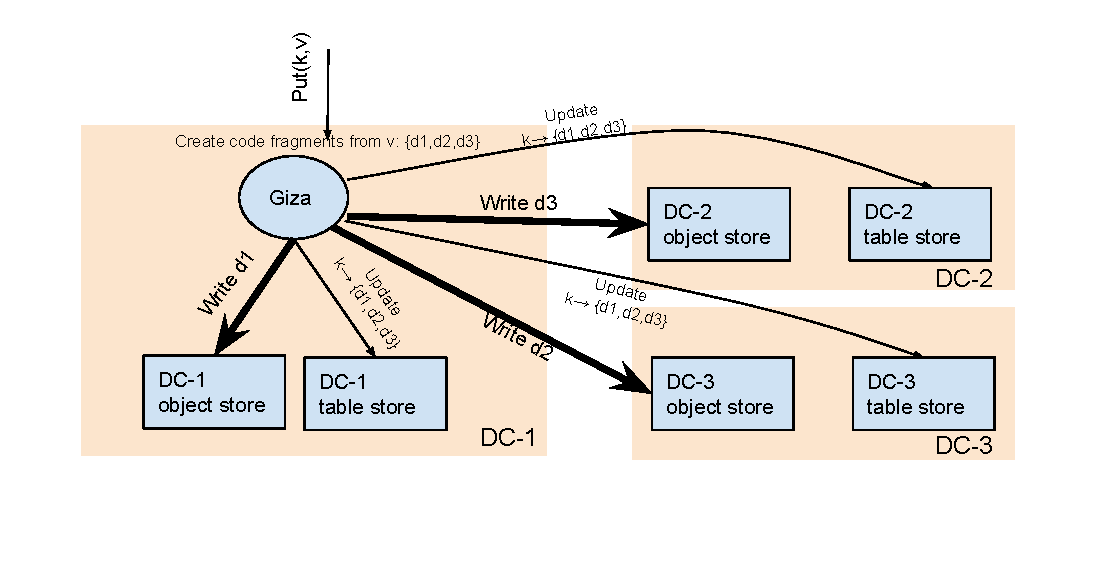
\includegraphics[width=0.5\textwidth]{fig/Giza}
\caption{Giza architecture\label{fig:arch}}
\end{figure}

\paragraph{Architecture}
{\name} is a global-scale cloud storage system 
that spans across many data centers in the world.
It stores mutable, versioned objects.
Figure~\ref{fig:arch} shows the architecture of \name. 
\name separates data path from meta-data path.
On the data path, \name splits and encodes the object into data and parity fragments.
Each fragment is uniquely named by it content hash
and stored in a different DC.
Updates to the object create new versions.
The version numbers, together with the names and the locations of the coded fragments in each version,
consist the meta-data of the object.
On the meta-data path, \name replicates the meta-data across multiple DCs.

We take the approach to layer \name on top of existing cloud storage infrastructure. This 
provides two advantages.  First, doing so allows the rapid development of \name by re-using 
mature, deployed systems.  Second, it simplifies the failure recovery and 
the deployment of \name, as \name nodes are completely stateless and can be
readily integrated with the rest of the stateless cloud storage front-ends.

%Existing cloud storage systems have redundancy within a single data center, but are not geo-replicated.  Thus, \name must explicitly provide cross data center redundancy through coding and replication.
To write the object,
{\name} stores the coded fragments in different data centers in {\em cloud blob stores},
such as Azure Blob, or AWS S3.
Additionally, \name replicates the object's meta-data across multiple data centers 
and stores the metadata in {\em cloud tables}, such as Azure Table, or AWS DynamoDB. 
The number of the coded fragments, and thus the set of data centers
storing the data object, is configurable depending on the user desired tradeoff on
durability vs. cost.
%The number of data centers to replicate the meta-data is fixed at 3.

%blob service as building blocks, to store metadata and data respectively. This evolutional
%design allows {\name} to minimize footprint of new code. In fact, {\name} merely needs to replace the previous front-end
%module. With {\name} deployed, the user request comes in to the new frontend, where the new
%{\name} service will translate the user requests into a few metadata operations and data operations.
%
%In {\name}, both metadata and data are synchronously duplicated across different
%datacenters in order to tolerate datacenter failures. What is different between metadata
%and data is, metadata is fully replicated across a (usually smaller) set of datacenters using
%a tailored Fast-Paxos algorithm, persistent in the table service in each datacenter, thus
%tolerating a minority of failures; On the other hand, data in user request is encoded to
%a configurable number of fragments and shipped to a (usually larger) set of datacenters,
%persistent in the blob storage service. We refer the former as metadata path and the latter
%as data path.


\paragraph{Technical challenges}
The data path of Giza is greatly simplified by naming the coded fragments by their content hashes.
Now, the coded fragments become immutable, as updating the object would result in completely different fragments and hashes.
Hence, storing immutable fragments in the cloud blob stores makes the data path straightforward.

On the other hand, the metadata path of Giza is rather subtle.
In designing \name, we address three main technical challenges involving the metadata path.
\begin{enumerate}

\item {\it Building a strongly consistent, geo-replicated meta-data storage out of existing 
single-DC cloud tables.}
There are existing solutions, such as Cassandra and CockcoarchDB,
that offer strongly consistent, geo-replicated storage systems.
Giza chooses not to adopt the existing solutions because
1) it is desirable to make \name nodes stateless and keep all data and meta-data
in existing cloud storage infrastructure;
2) it is preferable to implement protocols best suited for our targeted workloads,
so as to achieve optimal latency.
Indeed, Giza ensures strong consistency by implementing the Paxos consensus protocol.
But, how to implement Paxos using existing cloud storage APIs and achieve 
optimal latency in the cross-DC setting?

\item {\it Jointly optimizing the data and meta-data paths to achieve a single
cross-DC round trip for read/write operations.}
A naive approach would treat the data and metadata path sequentially:
a \name node completes the data path first before starting on the meta-data path.
While doing so guarantees that data is durably written at multiple DCs
before it becomes externally visible, each write operation requires at least two cross-DC round trips.
Similarly, a naive approach for read operation would take the first cross-DC round trip to retrieve the metadata
and then the second round trip to retrieve the data.
Can \name combine the data and metadata path operations to achieve a single cross-DC round trip for both read and write?

\item {\it Performing garbage collection efficiently and promptly.} 
\ch{Revisit later.}
When data is over-written and deleted, \name must remove obsolete data and/or meta-data from
the underlying cloud storage.  This is non-trivial because \name's garbage 
collection mechanism must be able to handle DC failures while ensuring data 
consistency and durability.

\end{enumerate}

%The separation of metadata path and datapath bring in the challenge that the consistency level
%could be violated with brutal yet flawed merge of the two. Our protocols described in later
%sections will guarantee the metadata path and data path together (especially when they are
%fully concurrent) will still provide a strong consistency insurance.
%


% A typical giza architecture for a data center includes the giza nodes, the Azure Blob Storage, and the Azure Table Storage. The giza nodes are the processing units of the Giza architecture and manages the data and the metadata. Furthermore the giza nodes participate in paxos rounds as coordinators. Figure 1 illustrates the architecture of Giza. Giza separates data from metadata and handles them on different paths. The data path is responsible for encoding the data and sending the data fragments across data centers. Each data fragment is stored in the corresponding DC’s Azure Blob Storage. The metadata path is responsible for storing the latest version of the data and the location of its data fragments. Giza uses a variant of the Paxos state machine replication (SMR) to maintain consistency of the metadata where each metadata server maintains a local copy of the replicated log. The replicated log is stored in the Azure Table Storage.

\subsection{Implementing Paxos using Cloud Storage APIs}

On the meta-data path, \name implements the Paxos consensus protocol on top of existing cloud tables,
such as Azure Table, or AWS DynamoDB.

\begin{figure}[tp]
\centering
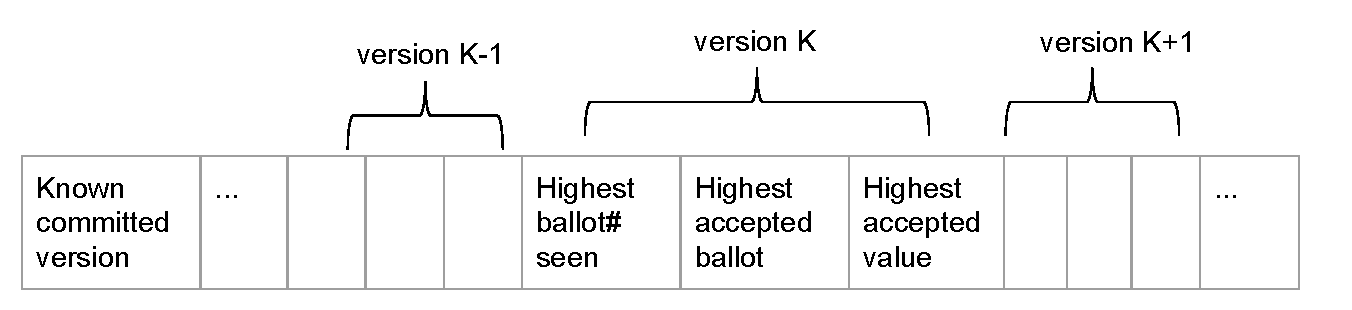
\includegraphics[width=0.5\textwidth]{fig/Giza_Metadata}
\caption{For each object, \name stores the Paxos protocol state and the object meta-data 
in a single row in the underlying cloud table.\label{fig:metadata}}
\end{figure}

\subsubsection{Meta-data Storage Layout}

\name implements the Paxos consensus protocol to serialize the operations on each data object.
Thus, it needs to persist the states of Paxos protocol in addition to the metadata for the object.
{\name} conveniently stores the Paxos states together with the metadata in the cloud table,
one table row per object, with a dynamic number of columns. The layout of each table row is
shown in Figure~\ref{fig:metadata}.

Each \name write operation leads to a new object version.
For each version, Giza invokes a separate Paxos instance to ensure consistency
in the event of races among multiple writers and failures.
The states of multiple Paxos instances, one instance per version, are stored in the same table row,
as part of the metadata for the data object.
Specifically, the meta-data contains a triplet of columns for each version of the object
(Figure~\ref{fig:metadata}).
%The triplet includes {\tt highest\_proposal\_seen}, {\tt highest\_accepted\_proposal}, and {\tt highest\_accepted\_value}.
The triplet includes {\tt highest proposal seen} and {\tt highest accepted proposal},
which are necessary fields recording the states of each Paxos instance.
The triplet also includes {\tt highest accepted value},
which contains the meta-data information for the erasure coding scheme,
the name of each coded fragment, whether it is one of the original or parity fragments,
and which DC the fragment is stored at. 

{\name} additionally maintains a set of {\tt known committed versions} for all the 
version numbers that have been committed by Paxos. As will become clear later,
this set provides a hint to facilitate both write and read operations.
It is a hint in the sense that newly committed versions are added to the set asynchronously,
or beyond the critical path of write operations.
Hence, while all the version numbers in the set are guaranteed to have been committed,
the latest committed version number might yet have to be included.

\subsubsection{Paxos vs. Fast Paxos}

Giza implements two consensus algorithms: Paxos and Fast Paxos. In general, Paxos requires two {\em phases} to reach consensus. Since each phase takes one round trip, applying Paxos in Giza results in two cross-DC round trips for metadata writes~\footnote{Typical Paxos optimization elects a distinguished leader. The leader executes {\em phase} $1$ in advance and only takes one round trip in {\em phase} $2$ to reach consensus. This, however, requires relaying all updates through the leader. In the cross-DC scenario, for metadata writes originating in non-leader DCs, it takes one cross-DC round trip to relay the writes to the leader. Therefore, these metadata writes still take two cross-DC round trips.}.

Fast Paxos, on the other hand, takes single round trip to reach consensus. It, however, requires a larger quorum than Paxos. Consider replicating the metadata across $3$ data centers, Paxos reaches consensus and completes the metadata replication when 2 out of the 3 data centers succeed. In comparison, Fast Paxos only reaches consensus and completes when all the 3 data centers succeed.

The requirement of a larger quorum in Fast Paxos turns out not an issue. Giza requires at least 3 data centers to stripe the coded fragments (with 2 + 1 erasure coding). Hence, the data path won't succeed unless there are at least 3 data centers available, which naturally satisfy the quorum requirement in Fast Paxos.

Hence, the most optimized metadata path in Giza implements Fast Paxos, as detailed next.

\subsubsection{Meta-data Write - Common Case}
The metadata path begins with choosing a proper new version number to run the Fast Paxos~\cite{fastpaxos} algorithm.
Version numbers are consecutive natural numbers, so the new version number needs to be next to the most recently committed version.
While it is safe to use an outdated version
(in which case the {\name} node will later realize its mistake and retry with a higher version number),
it is unsafe to choose a higher one and leaves holes in the version numbers.
The {\name} node identifies the proper version in an optimistic fashion.
Specifically, it reads {\tt known committed versions} from the table in its local DC,
then uses the next higher number as the chosen version number to invoke the corresponding Fast Paxos instance.

With the version number chosen, the {\name} node replicates a PreAccept request
to the tables in all the DCs.
Each request is an {\em atomic conditional update} to the corresponding table in a single DC.
If there are no competing requests on the same version, the PreAccept request will succeed in updating the table row.
Otherwise, the PreAccept request will be rejected by the table and leave the table row unchanged.
Section~\ref{sec:implementation} illustrates how atomic conditional update is implemented leveraging existing cloud APIs.

Whenever the {\name} node receives a {\em fast quorum} of positive PreAccept responses,
the corresponding version is considered to have been committed.
The {\name} node asynchronously replicates a Commit confirmation to all the DCs to update 
the set of {\tt known committed versions} to include the recently committed version.
The Commit confirmation is again an atomic conditional update,
which only succeeds if the version number is not yet included in the current set.

Since the Commit confirmation is completed asynchronously,
the critical path only involves the PreAccept request and response.
Hence, the above described metadata write involves only one cross-DC round trip 
and is referred to as the {\em fast path}.  When there is no
contention, the fast path always succeeds.

\subsubsection{Meta-data Write with Contention}

In the case of contention, the fast path may not succeed, i.e. the {\name} node
cannot collect a fast quorum of positive PreAccept responses. The contention
may come from concurrent updates to the same version, or a {\name} node trying
to recover from failures by re-committing the same or a different value to an
ongoing version.  In this case, {\name} enters what is referred to as a
\emph{slow path} to perform classic Paxos in order to guarantee safety in case of
contention.

On the slow path, the {\name} node first picks a distinguished ballot number
and then replicates a Prepare request to write the ballot to all the metadata
tables and wait for a majority of responses.
The Prepare request is a conditional update operation.
The operation succeeds only if the {\tt highest ballot seen} is no more than 
the ballot in the Prepare request.
The operation also returns the entire row as a result.

Upon collecting a majority of successful replies, the {\name} node needs to pick a value to commit.
The rule for picking the value is categorized into three cases.
In case 1, Giza looks for the highest accepted ballot in the replies.
If there is one, the value from the reply is picked.
In case 2, the replies contain no accepted value, but rather pre-accepted values.
Giza picks the pre-accepted value that appears more than others (if any) from the replies.
Both case 1 and 2 imply the possibility of an ongoing Paxos instance,
so Giza picks the value so as to complete the Paxos instance first.
It then starts with a new version and follows the fast path to commit its current metadata.
In case 3, there is neither pre-accepted nor accepted value,
which implies no real impact from contention.
Giza picks its current metadata as the value and proceeds to next steps.

Once the {\name} node picks a value, it replicates an Accept request to all the metadata tables.
The accept request is again an atomic conditional update; it succeeds in writing {\tt
highest accepted ballot} and {\tt highest accepted value} if neither {\tt
highest ballot seen} and {\tt highest accepted ballot} is larger.
As soon as a majority of Accept requests succeed, the \name node considers the
corresponding meta-data write completed and sends acknowledgment to clients.
Additionally, a Commit confirmation is replicated in the background, as described before.

\subsubsection{Metadata Read}

To get the metadata of the \emph{latest} object version,
it is insufficient for Giza to only read the corresponding metadata table row from its local DC.
This is because the local DC might not be part of the majority quorum that has accepted the latest version.
To ensure correctness, Giza needs to read the metadata rows from more than one DC.

In the common case,
{\tt known committed versions} is already updated and includes the latest committed version (say version $k$).
The metadata table row from the local DC obtains version $k$.
And the metadata table row from a non-local DC confirms the lack of higher committed versions than $k$.
Hence, in the case that the metadata is replicated to 3 DCs,
the metadata from 2 DCs (one local and one non-local) leads to a decisive conclusion that version $k$ is the latest committed version.
It is therefore safe for the Giza node to return version $k$ to clients.

In general, the \name node reads the metadata table rows from all the DCs.
Whenever a majority rows have matching {\tt known committed versions}
and have not accepted any value for a higher version, 
the \name node returns the metadata of the highest committed version.

If unfortunately the replies contain a higher version with accepted value while not included in {\tt known committed versions},
the \name node needs to follow a slow path similar to the one in the write operation.
This is to confirm whether the higher version has indeed been committed,
despite that the version is not included in {\tt known committed versions} and the metadata tables in certain DCs may have missed the quorum.

%This is because it could possibly be considered committed once before. After it succeed in the slow path, the {\name} node needs to re-launch the datapath to retrive the data fragments of the newer version and abandon the old ones. This serialized metadata and datapath case typically happens when there is concurrent read and write on the same object, which is rare in our workload.

%\sm{ Hi Daniel, just want to confirm, is this what you do now? Only one accepted in higher version will invalidate the optimistic read}

% continue to design_part2.tex

\subsection{Joint optimization of Data and Meta-date Operations}

The data path of \name is straightforward: the \name node encodes the data to $k$ original
fragments and $m$ parity fragments. $k$ and $m$ are configurable. Then the Giza node
computes a content hash for each fragment, and uses the hash value as the key to
write each fragment to a separate data center.
When naively combining the data path with the earlier metadata path,
the \name node serializes the two paths, resulting in two or more cross-DC round trips.
To reduce latency, we optimize \name to run the data and metadata paths in parallel.
This is potentially problematic because either the data or metadata path could fail
while the other one succeeds.
Below, we describe how {\em put} and {\em get} cope with this challenge and ensure end-to-end correctness.

\comment{

{\name} supports three operations: put, get and delete. All of them require a key as
an argument to identify an object. put takes object content as an extra argument, get
returns object content (null if non-exist) as result. A delete operation is processed
as a special write, putting a tombstone in the object's metadata. The actual recycling
of disk space happens at garbage collection, which will be described in ~\Cref{sec:xxxx}.

}

{\bf The Put Operation:}
After generating the coded fragments and calculating their content hashes,
the \name node launches both the data and metadata paths in parallel.
In the common case,
the \name node waits for both the data and the metadata paths to finish before acknowledging clients.
Furthermore, it replicates the Commit confirmation only after both the data and the metadata paths complete. 
In other words, \name ensures that {\tt known committed version} only include those versions
whose data and metadata have both been successfully committed.

In one uncommon case, the data path succeeds, while the metadata path fails.
Now, the fragments stored in the cloud blobs become useless.
Giza deletes these fragments and reclaims storage through a cleaning process,
which first executes Paxos to update the current version to {\em no-op}
and then removes the fragments from the corresponding blob stores in all the DCs.

In another uncommon case, the data path fails, but the metadata path succeeds.
This is rather subtle, as it creates a challenging for the {\em get} operation,
as addressed next.

{\bf The Get Operation:}
A naive way to perform {\em get} is to first read the latest metadata and then retrieve the coded fragments.
To reduce latency, {\name} chooses an optimistic approach and parallelizes the metadata and the data paths.

For a {\em get} request, the {\name} node first reads from the local DC the corresponding metadata table row.
It obtains {\tt known committed version}, as well as the names and locations of the coded fragments of the latest version.
The \name node immediately starts reading the coded fragments from the different data centers.
Separately, it launches a regular metadata read to validate that the version is indeed the latest.
If the validation fails, the \name node realizes there is a newer version.
It in turn has to redo the data path by fetching a different set of coded fragments.
This results in wasted efforts in its previous data fetch.
Such potential waste, however, only happens when there is concurrent writes on the same object,
which is rare.

Because the data and metadata paths are performed in parallel during {\em put},
it is possible (though rare) that the coded fragments for the latest committed version
have not been written to the blob storage at the time of read.
This happens if the metadata path in the {\em put} finishes before the data path,
or the metadata path succeeds while the data path fails.
In such case, the {\name} node needs to fall back to read the previous version,
as specified in {\tt known committed version}.

\comment{

\sm {
  Hi Daniel, can you give me a few details about the hashing? e.g. hashing method,
  hashing result size, collision rate, etc.)
}

}

\subsection{Deletion and Garbage Collection}

Giza supports two types of deletion operation: trimming earlier versions and deleting entire data object.
To control the size of the metadata table rows, Giza limits the number of versions for each object.
Once the limit is reached, writing a new version automatically trims the earliest version.

Deleting a specific version is processed as a special update of the object's metadata.
It again executes the Paxos algorithm and creates a new version to record a deletion record for the deleted version.
Once the deletion record is successfully committed,
Giza garbage collects and reclaims the storage spaced occupied by the coded fragments of the deleted version.

\comment{
Because {\name} keeps writing new version metadata to table service and data fragments
to blob storage service, it needs to garbage collect on outdated versions to recycle
storage space. Moreover, the garbage collection also needs to free the space marked as
tombstone by the delete operation.
}

The garbage collection process includes deleting the coded fragments and
truncating the column for the deleted version in the metadata table row.
It follows three steps:
1) read the metadata row and identify the column corresponding to the deleted version;
2) send deletion requests to blob storage to delete the coded fragments;
3) remove the column for the deleted version from the table storage.
The second step has to occur before the third one in case that
the garbage collection process is interrupted and the coded fragments may become ``orphans''
without proper metadata pointing to them in the table storage.

To delete the entire object, 
{\name} first executes Paxos to commit a tombstone as the highest version.
Then, it deletes the coded fragments corresponding to all the versions of the object.
Finally, it starts to delete the entire table row from the tables across all the DCs.
This requires extra care. Otherwise if removed brutally, 
a new {\em put} operation of the same object may lead the system into an abnormal state.
The {\em put} operation could start at a data center where the table row is already deleted.
The {\em put} operation would therefore assume the object never existed and choose the smallest version number.
Committing this version number could be dangerous before the metadata table row is deleted from all the DCs,
as this could result in conflict and ambiguity during future failure recovery.

% start with an initial version, which could violate some of the metadata (with a higher version before the deletion) if the removing is still in process.
Therefore, {\name} resorts to two-phase commit to delete the metadata table row.
In the first phase, it marks the rows in all the data centers as ``prepared\_to\_delete''.
After this any other {\em get} or {\em put} operations are temporarily disabled on this object.
Then in the second phase, all the rows are actually removed from the table storage.
The disadvantage of this approach is that it requires all the data centers online.
Data center failure or network partition may pause the process and make the row unavailable
(but can still continue after data center recovers or network partition heals). 



% \subsection{Giza Workflow}
% Because of the high WAN RTT, Giza’s primary goal is to minimize the number of round trips in its put and get critical paths while maintaining strong consistency semantics. By approaching this problem with multiple iterations, we were able to reduce the original 3  WAN RTT to 1 WAN RTT in most cases, dramatically reducing the put and get latency.

% \subsubsection{3 RTT Put and Get}
% Figure 3 illustrates the workflow of a typical Put operation. When a client issues a Put command, Giza first queries its local metadata to identify a most likely latest version of the object. It then starts a paxos round for the version. A paxos round is broken down into two phases: the prepare phase and the accept phase. Giza runs the data path first, where the object is erasure encoded and the data fragments are sent to the corresponding data centers. (Here, we have to write this information down in case of giza node failure right). When the data path returns successfully, Giza proceeds to run the metadata phase which incurs two round trips.
% \par 
% During the Get path, Giza runs the metadata phase first to get the location of the data fragments. To ensure a consistent latest version of the data, Giza runs a paxos round for get on the object’s entry log. When this succeeds, Giza runs the datapath and receives enough data fragments to reconstruct the original data before returning to the client. Both the Put and Get incurs two rounds in the metadata path and 1 round in the data path.

% \subsubsection{2 RTT Put and Get}
% We quickly realized that the separation of metadata path and data path allows for some parallelism. In particular, during the Put path, Giza can run the prepare phase of the metadata path in parallel with the data path. When prepare phase and the data path succeed, Giza runs the second phase of the paxos round. Once this round completes, Giza can return acknowledgement to the client. This brings the round trips down to 2 round trips in the optimal case.
% \par
% Furthermore, during Get, Giza can run the additional paxos round for the get operation in parallel with the data path get. This can be done by first optimistically assuming that the current highest entry of the object in its local entry log is in fact the highest version. Once this information is obtained, Giza can then proceed to get the data fragments while simultaneously validating the consistency of the latest version on the metadata path. If the assumption is correct, the Get incurs 2 round trips.

% \subsubsection{1 RTT Put and Get}
% We used the classical Paxos protocol for achieving consistency on our metadata path. [Introduce Fast Paxos and why this works in this case, should do this after reading in depth about Fast Paxos]. This reduces Giza’s put path to 1 round trip.
% \par
% In the Get Path, we realized that we can forego running the paxos round in some scenarios by including a learning phase on the non-critical path of Put. After acknowledging to the client’s put request, the coordinator giza node will send the accepted version and the version number as a committed entry for the object to the other participating giza nodes. This entry is used to serve as the highest committed version and will only override existing entry if the version is higher. During a client’s Get request, Giza first obtains the object’s row entry from the majority of the participating giza nodes. If the latest entry in the paxos log are consistent or not higher than the highest committed entry, then Giza can safely return the results obtained from the data path. However, in the case where the latest entry in the paxos log is higher than the highest committed entry (This can happen if the giza nodes are simultaneously performing a paxos round for a newer version of the object or the learning phase has not reached the giza nodes), then Giza can still get the highest version but doing two things. First it can fallback to the previous approach of running a paxos round for the get operation. Alternatively, it can wait to obtain the object’s row from all the participating giza nodes (instead of the previous majority). In our scheme, we execute both options concurrently and return once the faster of the two approaches completes.

% \subsection{Giza Recovery}
% Describe the mechanism of recovery when a data path node fails but a metadata path node doesn’t (6-1 scheme still only utilizes 3 giza nodes for metadata).
% \par
% Describe the mechanism when a DC containing both data path and metadata path node fails (membership change).

%%% Local Variables:
%%% mode: latex
%%% TeX-master: "main"
%%% End:


\section{Reconfiguration}
This section discusses about relatively rare cases that happen in {\name}
and how {\name} handle these cases. Because the main protocols are designed
to guarantee safety with contention and any minority of failures, it is much
easier to handle cases such as failure recovery, viewchange, migration etc.
\subsection{Failure Recovery}

Failures in {\name} are mainly in two catogeries: {\name} node failures and
datacenter failures. If a {\name} node stops responding or is malfunctioning,
we simply launch a new machine to take over its responsibility, and send a
signal to shut it down. Note that the new node does not need to wait until
the shutdown to finish. That said, both the new and previous nodes could be
alive in the systems. This is okay because the {\name} protocols already
guarantee safety in case of contention, thus no particular actions needed
to force the end of life cycle of the malfunctioning node (which might not
respond to any signals at all since it is malfunctioning).

{\name} assumes the table service and blob storage service are reliable.
Any errors related to these, e.g. unable to read or write, are considered
as datacenter failures in {\name}. These failures can be caused by multiple
reasons, such as a temporary network partition or an entire datacenter breakdown.
In such cases {\name} can still make progress as long as there are enough
datacenter left. It is worth noticing that the threshold could be different for
metadata path and data path. For metadata, a majority of alive datacenters
are required. For data path, assume it writes to $N$ datacenters in total with
$m$ data fragments. To tolerate $F$ datacenter failures, it needs to write
to at least $F+m$ datacenters, which implies that $F<N-m$ (To tolerate $F$
failures, you need to have at least $F$ parities).

When a datacenter comes back online after crash, it needs to update the
metadata rows in its table service and data fragments in the blob storage.
A number of recovering clients are launched to scan through its objects.
For each object, it issues a normal read request except that it does not
pre-fetch the data. If the local version match the global version, nothing
needs to be done; if the local version is behind, the recovering process
then reads the latest data fragments, re-calcuates the fragment that belongs
to the local datacenter and writes it to the blob storage consistently with
the metadata.

\subsection{View change}
Each {\name} account has a \emph{view}, which stores membership information
including the datacenter set to replicate metadata and the set to store the
data fragments. The view is created when the storage account is created,
assigned by user preferences. For example, an OneDrive-like application may
create a number of {\name} accounts, each of which stores data for users
in a geographical region. The application could set up these accounts to
choose a few datacenters that are close to that region for better user
experience.

Occasionaly {\name} users might need to change the view to a different set
of datacenters. For instance, a datacenter might have permanently crashed,
or the application simply wants to use a faster location. For each storage
account, {\name} stores the view as a special key in the metadata table.
When it receives a viewchange request, {\name} goes into a gracing period.
In this period, it writes the new view to the metadata table and tries to
invalidate the cache in all {\name} nodes. In the gracing period, it is
possible that different nodes hold different views. They may read or write
different set of datacenters. If a {\name} node fails with its current
view, it re-reads the most recent view and recursively retries. To make it
faster, a view version id is also attached to each object's metadata.
Since view change happens rarely, we keep history of all views.

In spite of metadata, view change also requires data migration. A number
of migration process are launched to move both the metadata and data to
the new set of datacenters. This is similar to the failure recovery process,
except that the migration process needs to update the view id in the
metadata. In case of coding reconfiguration, i.e. the application changes
the number of data fragments in encoding, the migration process also needs
to compute all the parity fragments for the new view.




\section{Implementation}
We implement Giza in C++ as a frontend on top of Microsoft Azure. We chose Azure because currently it provides the largest number of data centers across different geographical regions. This allows for experimenting with a wider range of coding schemes. However, Giza is designed to be invariant to the underlying cloud services and can be deployed by simply creating new interfaces to the specific table and blob storage. We implemented the Azure storage and table interface using the official Azure Storage Client Library for C++ (2.4.0). We use the Jerasure and GF-Complete erasure code libraries for coding the data using Reed-Solomon coding. However, Giza allows the flexibility for using different coding schemes as well.

Giza also serves as a frontend for other Giza nodes during table and blob storage accesses. When a Giza in a data center makes a request to the table and blob storage in another data center, it does by making an rpc call to the Giza node in the targeted data center. Hence, a Giza node does not directly interact with the table and blob storage in data centers located in other geographical regions. We made this implementation decision for two reasons. First, in ordere to implement the paxos logic using the underlying table interface, multiple requests might be necessary. This would incur unnecessary cross WAN round trips. In our case with Azure table, we implement the atomic updates to the paxos acceptors by using the provided Etags. When updating an acceptor entry, Giza first reads the entry and its associated etag. It then decides whether entry's value can be updated. If this is the case, Giza makes a replace entity request that only succeeds if the entry's etag value is still the same. During concurrent requests, this process can repeat multiple times. Second, we make the assumption that all network traffics are routed over the public internet. While this doesn't have to be the case since some cloud providers do offer dedicated private connection (e.g Azure Express Route), setting up private connections across wide area network may be too costly to be an option. As such, cross regional vm to storage latency performance can be significantly degraded during peak hours. We observed that latency can be reduced by first sending metadata and data to the vm of the targeted data center and then having the vm send data to its local blob and table storage. 


\section{Evaluation}
We benchmark Giza against CockroachDB, a globally distributed SQL database inspired by Google’s Spanner. Both CockroachDB and Giza share similar goals, mainly to provide strong consistency semantics to users while being able to tolerate data center outages. In addition, it is easy to implement the read and write path of Giza with database transaction. [But while we know this may not be a fair comparison since CockroachDB provides more functionality than Giza, we want to show that Giza cannot be implemented with existing systems].

What type of results are presented and what are we trying to show through these results? We use YCSB to generate the following workload:
- latency result from Giza and CockroachDB when there’s no read or write conflict. To show that if we were to choose an existing system and implement our scheme, our latency would still be better. 
Also to show 2-1 scheme, 7-1 scheme, and world wide scheme

- throughput and read latency graph of Giza. To show that we can tolerate contention when doing write heavy work.

qustions to answer?

performance with difference sized object and with different contention level.
 -latency result, single node throughput

correctness under failures/network partitions.
 

\subsection{Setup}
For all experiments, we deployed a single virtual machine (how many cores, how many whatever) for each geographical region to act as the front end for the regional data center. In addition, The virtual machines are deployed through the console provided by the cloud computing platform. 

How did we set up Giza?

We deployed both a table service and a blob service provided by the cloud platform for each geographical region. The granularity of replication for these services varies from provider to provider but we always choose the replication level to match that of the regional replication. This means that as long as there’s no dc outage, the data would not be lost. On top of each table service and blob service, we also run a front end interface for the table and blob service respectively. This is to avoid unnecessary WAN round trip when executing metadata path logic. The Giza node interacts with table and blob service front end via Thrift RPC calls, sending the appropriate metadata and data to other regions.  

How did we set up CockroachDB?

We run a CockroachDB cluster spanning all the data centers included in the experiment where each node correspond to the virtual machine running on each geographical region. We use a single database of CockroachDB to emulate our Giza read and write path. The database contains multiple tables, a metadata table and multiple data tables corresponding to their respective region, and the tables differ in their replication level. The metadata table is replicated according to the fault tolerance level, i.e 2 if the the cluster can tolerate one data center outage [what about the location?]. The data table is replicated once only at the node of the respective region.
*machines*

*workloads ycsb*

*performance metrics: latency, cpu*

*is it possible to choose real workload?*


\subsection{Small object}
64K $\sim$ 16MB

X-axis: Value size
Y-axis: 50\% Read latency

X-axis: Value size
Y-axis: 90\% Read latency

X-axis: Value size
Y-axis: 99\% Read latency

Same for write

[adding cpu results in a table]

\subsection{Large object}
256MB $\sim$ 1GB

X-axis: Value size
Y-axis: Average Read latency

X-axis: Value size
Y-axis: Average Write latency


\subsection{Contention}

Fixed object size
X-axis: zipf coefficient
Y-axis: 50\%, 90\%, 99\% Read/Write Latency


\subsection{Real workload}
Table.
%\realnewpage
\section{Related Work}

%%% Local Variables:
%%% mode: latex
%%% TeX-master: "main"
%%% End:

{\bf Erasure Coding in Cluster Storage:}
Erasure coding has long been applied in many large-scale distributed storage
systems~\cite{fab:asplos04, zhang04repstore, haeberlen05glacier, abd05ursa,
  welch08scalable, sathiamoorthy13xoring, zhang16efficient}, including
productions systems at Facebook~\cite{borthakur2010hdfs},
Google~\cite{fikes2010storage, ford10availability} and Microsoft
Azure~\cite{huang12erasure}. These solutions generalize the RAID
approach~\cite{patterson88case, wilkes96hp} to a distributed cluster setting.
Giza is unique in synchronously replicating erasure coded data across WAN
and minimizing cross-DC latency. In addition,
Giza provides globally consistent {\em put} and {\em get} with versioning support.

{\bf Erasure Coding in Wide Area Storage:}
HAIL~\cite{hail:ccs09}, OceanStore~\cite{oceanstore:asplos00, pond:fast03},
RACS~\cite{racs:socc10}, DepSky~\cite{depsky:eurosys11} 
and NCCloud~\cite{nccloud:fast12} all stripe and erasure code data at a global scale.

HAIL~\cite{hail:ccs09} is designed to withstand Byzantine adversaries.
OceanStore~\cite{oceanstore:asplos00, pond:fast03} assumes untrusted infrastructure
and serializes updates via a primary tier of replicas.
Giza operates in a trusted environment.

RACS~\cite{racs:socc10} and DepSky~\cite{depsky:eurosys11} address conflicts
caused by concurrent writers using Apache ZooKeeper~\cite{zookeeper:atc10},
where readers-writer locks are implemented at per-key granularity for synchronization.
Giza, on the other hand, implements consensus algorithms for individual keys
and achieves strong consistency without centralized coordinators.
In addition, Giza employs a leaderless consensus protocol. 
Updates may originate from arbitrary data centers
and still complete with optimal latency without being relayed through a primary.

NCCloud~\cite{nccloud:fast12} implements a class of functional regenerating
codes~\cite{dimakis07networkcoding} that optimize cross-WAN repair bandwidth.
Giza employs standard Reed-Solomon coding and leaves such optimization to future.

Facebook f4~\cite{f4:osdi14} is a production warm blob storage system.
It applies erasure coding across data centers for storage efficiency.
As discussed in Section~\ref{sec:alternative}, f4 avoids the
deletion challenge by never truly deleting data objects. 
Whenever a data object is deleted, the unique key used to encrypt the object is destroyed
while the encrypted data remains in the system.
This simplification suits Facebook very well, because its deleted
data only accounts for $6.8\%$ of total storage and Facebook could afford not to
reclaim the storage space~\cite{f4:osdi14}. This, unfortunately, is not an
option for Giza, as our workloads show much higher deletion rate. Not reclaiming
the physical storage space from deleted data objects would result in significant
waste and completely void the gain from cross-DC erasure coding. Furthermore,
not physically deleting customer data objects - even if encrypted - wouldn't
meet the compliance requirements for many of our customers.

\comment{
In comparison, Giza vastly simplifies the deletion problem by treating data
objects independently. It deletes a data object by deleting all its data and
parity fragments from individual DCs, which involves only tiny metadata traffic
across WAN. Given the necessity and simplicity to implement deletion, Giza
chooses to split individual data objects and incur WAN traffic and latency when
serving data. Since the target workload for Giza is rather cold (very small
numbers of reads over a large corpus of data), the amount of WAN traffic due to
serving data turns out only a small fraction compared to storing data.

There are two general approaches in applying erasure coding to storage.  One
is to generate coded fragments within each data object.  This is commonly used
to achieve redundancy within a single data center~\cite{f4:osdi14}.  Another 
approach is to treat multiple data objects as a coding group and generate
parity blocks that combine multiple objects.  Facebook's cross-DC erasure
coding uses this scheme to code immutable blobs.  To handle mutable coded
blocks, prior work resort to a RAID-like approach~\cite{zhang16efficient} of using
static coding groups comprising of fixed sized blocks. The RAID approach has
only been applied in cluster settings.
}

{\bf Separating Data and Metadata:}
It is common for a storage systems to separate data and metadata path, and
design a separate metadata service to achieve better scalability, e.g.,
FARSITE~\cite{adya02farsite} and Ceph~\cite{weil06ceph}.
Gnothi~\cite{wang12gnothi} replicates metadata to all replicas while data blocks
only to a subset of the replicas. Cocytus~\cite{zhang16efficient} is a highly
available in-memory KV-store that applies replication to metadata and erasure
coding to data so as to achieve memory efficiency. Giza follows a similar design
path, and store data in commodity cloud blob storage and metadata in commodity
NoSQL table storage.

{\bf Consistency in Global Storage:} 
Megastore~\cite{baker11megastore} and
Spanner~\cite{spanner:osdi12} applies Multi-Paxos to maintain strong consistency
in global databases. Both of them requires two round trips for a slave site to
commit. Mencius~\cite{mao08mencius} takes a round-robin approach for proposers in
different sites, amortizing commit latency. EPaxos~\cite{epaxos:sosp13} uses
fine-grained dependency tracking at acceptor-side to ensure low commit latency
for both non-contended and contended requests. In comparison, 
\name takes a refined approach based on FastPaxos~\cite{lamport05fast},
separating metadata and data path before committing. This design choice allows
\name to serve most requests still in single cross-DC round trip
while keeping servers stateless, using the limited ability of table service.
Metasync~\cite{metasync:atc15} implements Paxos using the append functionality
provided by cloud file synchronization services such as DropBox, OneDrive. By
contrast, Giza implements Paxos using conditional-write APIs of cloud tables.
The latter leads to a more efficient implementation as clients do not need to
download and process logs from the cloud storage in order to execute Paxos.

%%% Local Variables:
%%% mode: latex
%%% TeX-master: "main"
%%% End:


\section{Conclusion}

In this paper, we present the design and evaluation of Giza -- a strongly
consistent, versioned object store that encodes objects across global data
centers. Giza implements the Paxos consensus algorithms on top of existing cloud
APIs and have separate data and metadata paths. As a result, Giza is fast in
normal operation for our target workloads. Our evaluation of Giza on a
deployment over \deployment demonstrates that Giza achieves much lower latency
than naively adopting a globally consistent storage system.

\section{Acknowledgments}

We thank Andy Glover, Jose Barreto, Jon Bruso, Ronakkumar Desai, Joshua Entz from the OneDrive team for their many contributions.
Special thanks go to Jeff Irwin for his contributions that helped enable Giza.
We also thank all of the members of the Azure Storage team for invaluable discussions and iterations,
as well as Taesoo Kim and anonymous reviewers for their insightful feedback.

%\realnewpage
%\input{bg}
%%% \section{Overview}

%% [TODO put this to a separate file and come with a plan]

%% [Shall we put the assumptions/setup here?]

%% [Shall we put the interface here?]

%% [Give a table, summarize the interface]

%% % \subsection{Interface and Assumptions}
%%                                 % Giza is an erasure coding scheme for key/value stores and provide two operations: Put(Key, Value) and Get(Key), where Key and Value are arbitrary strings. Get(Key) returns the value of the latest Put for that key. (Add assumptions here + what giza is good for: Giza provides fault tolerance for non byzantine failures in an asynchronous network)


%% % operations  semantics
%% % put         
%% % get 
%% % get_stale

%% \subsection{State Machine Replication and Paxos}

%% \subsection{Erasure coding}

\section{Design}

This section presents the design of {\name}, including the overall architecture,
the data model, and the protocols for the {\em put}, {\em get} and {\em delete} operations.

\subsection{Overview and challenges}

\begin{figure}[tp]
\centering
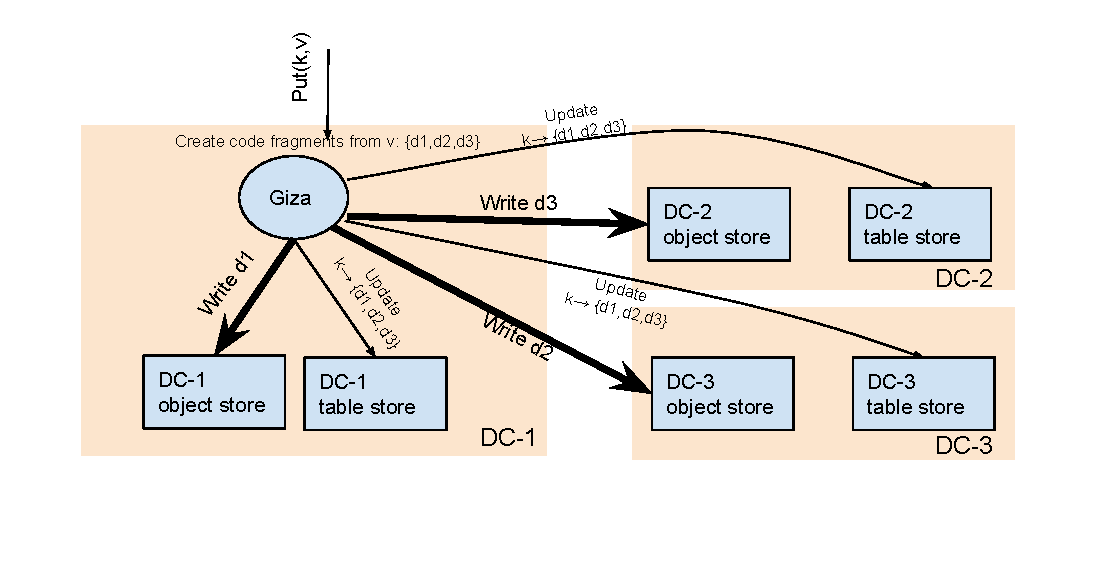
\includegraphics[width=0.5\textwidth]{fig/Giza}
\caption{Giza architecture\label{fig:arch}}
\end{figure}

\paragraph{Architecture}
{\name} is a global-scale cloud storage system 
that spans across many data centers in the world.
It stores mutable, versioned objects.
Figure~\ref{fig:arch} shows the architecture of \name. 
\name separates data path from meta-data path.
On the data path, \name splits and encodes the object into data and parity fragments.
Each fragment is uniquely named by it content hash
and stored in a different DC.
Updates to the object create new versions.
The version numbers, together with the names and the locations of the coded fragments in each version,
consist the meta-data of the object.
On the meta-data path, \name replicates the meta-data across multiple DCs.

We take the approach to layer \name on top of existing cloud storage infrastructure. This 
provides two advantages.  First, doing so allows the rapid development of \name by re-using 
mature, deployed systems.  Second, it simplifies the failure recovery and 
the deployment of \name, as \name nodes are completely stateless and can be
readily integrated with the rest of the stateless cloud storage front-ends.

%Existing cloud storage systems have redundancy within a single data center, but are not geo-replicated.  Thus, \name must explicitly provide cross data center redundancy through coding and replication.
To write the object,
{\name} stores the coded fragments in different data centers in {\em cloud blob stores},
such as Azure Blob, or AWS S3.
Additionally, \name replicates the object's meta-data across multiple data centers 
and stores the metadata in {\em cloud tables}, such as Azure Table, or AWS DynamoDB. 
The number of the coded fragments, and thus the set of data centers
storing the data object, is configurable depending on the user desired tradeoff on
durability vs. cost.
%The number of data centers to replicate the meta-data is fixed at 3.

%blob service as building blocks, to store metadata and data respectively. This evolutional
%design allows {\name} to minimize footprint of new code. In fact, {\name} merely needs to replace the previous front-end
%module. With {\name} deployed, the user request comes in to the new frontend, where the new
%{\name} service will translate the user requests into a few metadata operations and data operations.
%
%In {\name}, both metadata and data are synchronously duplicated across different
%datacenters in order to tolerate datacenter failures. What is different between metadata
%and data is, metadata is fully replicated across a (usually smaller) set of datacenters using
%a tailored Fast-Paxos algorithm, persistent in the table service in each datacenter, thus
%tolerating a minority of failures; On the other hand, data in user request is encoded to
%a configurable number of fragments and shipped to a (usually larger) set of datacenters,
%persistent in the blob storage service. We refer the former as metadata path and the latter
%as data path.


\paragraph{Technical challenges}
The data path of Giza is greatly simplified by naming the coded fragments by their content hashes.
Now, the coded fragments become immutable, as updating the object would result in completely different fragments and hashes.
Hence, storing immutable fragments in the cloud blob stores makes the data path straightforward.

On the other hand, the metadata path of Giza is rather subtle.
In designing \name, we address three main technical challenges involving the metadata path.
\begin{enumerate}

\item {\it Building a strongly consistent, geo-replicated meta-data storage out of existing 
single-DC cloud tables.}
There are existing solutions, such as Cassandra and CockcoarchDB,
that offer strongly consistent, geo-replicated storage systems.
Giza chooses not to adopt the existing solutions because
1) it is desirable to make \name nodes stateless and keep all data and meta-data
in existing cloud storage infrastructure;
2) it is preferable to implement protocols best suited for our targeted workloads,
so as to achieve optimal latency.
Indeed, Giza ensures strong consistency by implementing the Paxos consensus protocol.
But, how to implement Paxos using existing cloud storage APIs and achieve 
optimal latency in the cross-DC setting?

\item {\it Jointly optimizing the data and meta-data paths to achieve a single
cross-DC round trip for read/write operations.}
A naive approach would treat the data and metadata path sequentially:
a \name node completes the data path first before starting on the meta-data path.
While doing so guarantees that data is durably written at multiple DCs
before it becomes externally visible, each write operation requires at least two cross-DC round trips.
Similarly, a naive approach for read operation would take the first cross-DC round trip to retrieve the metadata
and then the second round trip to retrieve the data.
Can \name combine the data and metadata path operations to achieve a single cross-DC round trip for both read and write?

\item {\it Performing garbage collection efficiently and promptly.} 
\ch{Revisit later.}
When data is over-written and deleted, \name must remove obsolete data and/or meta-data from
the underlying cloud storage.  This is non-trivial because \name's garbage 
collection mechanism must be able to handle DC failures while ensuring data 
consistency and durability.

\end{enumerate}

%The separation of metadata path and datapath bring in the challenge that the consistency level
%could be violated with brutal yet flawed merge of the two. Our protocols described in later
%sections will guarantee the metadata path and data path together (especially when they are
%fully concurrent) will still provide a strong consistency insurance.
%


% A typical giza architecture for a data center includes the giza nodes, the Azure Blob Storage, and the Azure Table Storage. The giza nodes are the processing units of the Giza architecture and manages the data and the metadata. Furthermore the giza nodes participate in paxos rounds as coordinators. Figure 1 illustrates the architecture of Giza. Giza separates data from metadata and handles them on different paths. The data path is responsible for encoding the data and sending the data fragments across data centers. Each data fragment is stored in the corresponding DC’s Azure Blob Storage. The metadata path is responsible for storing the latest version of the data and the location of its data fragments. Giza uses a variant of the Paxos state machine replication (SMR) to maintain consistency of the metadata where each metadata server maintains a local copy of the replicated log. The replicated log is stored in the Azure Table Storage.

\subsection{Implementing Paxos using Cloud Storage APIs}

On the meta-data path, \name implements the Paxos consensus protocol on top of existing cloud tables,
such as Azure Table, or AWS DynamoDB.

\begin{figure}[tp]
\centering
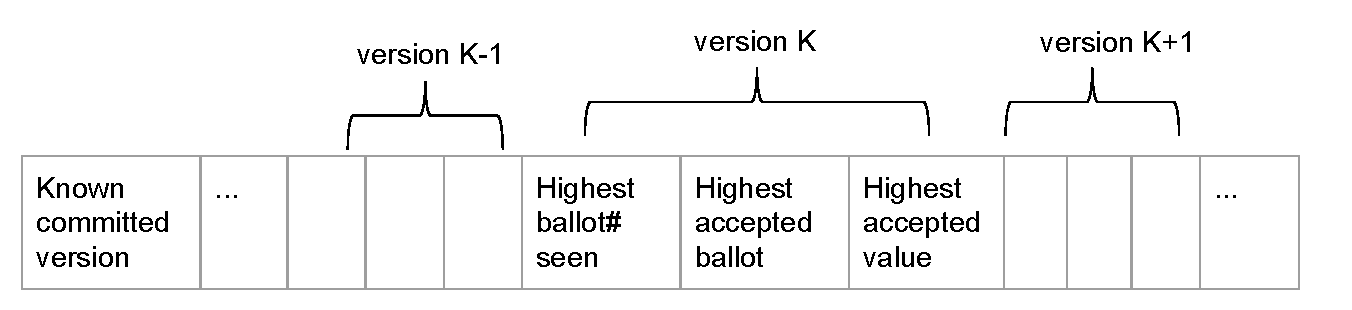
\includegraphics[width=0.5\textwidth]{fig/Giza_Metadata}
\caption{For each object, \name stores the Paxos protocol state and the object meta-data 
in a single row in the underlying cloud table.\label{fig:metadata}}
\end{figure}

\subsubsection{Meta-data Storage Layout}

\name implements the Paxos consensus protocol to serialize the operations on each data object.
Thus, it needs to persist the states of Paxos protocol in addition to the metadata for the object.
{\name} conveniently stores the Paxos states together with the metadata in the cloud table,
one table row per object, with a dynamic number of columns. The layout of each table row is
shown in Figure~\ref{fig:metadata}.

Each \name write operation leads to a new object version.
For each version, Giza invokes a separate Paxos instance to ensure consistency
in the event of races among multiple writers and failures.
The states of multiple Paxos instances, one instance per version, are stored in the same table row,
as part of the metadata for the data object.
Specifically, the meta-data contains a triplet of columns for each version of the object
(Figure~\ref{fig:metadata}).
%The triplet includes {\tt highest\_proposal\_seen}, {\tt highest\_accepted\_proposal}, and {\tt highest\_accepted\_value}.
The triplet includes {\tt highest proposal seen} and {\tt highest accepted proposal},
which are necessary fields recording the states of each Paxos instance.
The triplet also includes {\tt highest accepted value},
which contains the meta-data information for the erasure coding scheme,
the name of each coded fragment, whether it is one of the original or parity fragments,
and which DC the fragment is stored at. 

{\name} additionally maintains a set of {\tt known committed versions} for all the 
version numbers that have been committed by Paxos. As will become clear later,
this set provides a hint to facilitate both write and read operations.
It is a hint in the sense that newly committed versions are added to the set asynchronously,
or beyond the critical path of write operations.
Hence, while all the version numbers in the set are guaranteed to have been committed,
the latest committed version number might yet have to be included.

\subsubsection{Paxos vs. Fast Paxos}

Giza implements two consensus algorithms: Paxos and Fast Paxos. In general, Paxos requires two {\em phases} to reach consensus. Since each phase takes one round trip, applying Paxos in Giza results in two cross-DC round trips for metadata writes~\footnote{Typical Paxos optimization elects a distinguished leader. The leader executes {\em phase} $1$ in advance and only takes one round trip in {\em phase} $2$ to reach consensus. This, however, requires relaying all updates through the leader. In the cross-DC scenario, for metadata writes originating in non-leader DCs, it takes one cross-DC round trip to relay the writes to the leader. Therefore, these metadata writes still take two cross-DC round trips.}.

Fast Paxos, on the other hand, takes single round trip to reach consensus. It, however, requires a larger quorum than Paxos. Consider replicating the metadata across $3$ data centers, Paxos reaches consensus and completes the metadata replication when 2 out of the 3 data centers succeed. In comparison, Fast Paxos only reaches consensus and completes when all the 3 data centers succeed.

The requirement of a larger quorum in Fast Paxos turns out not an issue. Giza requires at least 3 data centers to stripe the coded fragments (with 2 + 1 erasure coding). Hence, the data path won't succeed unless there are at least 3 data centers available, which naturally satisfy the quorum requirement in Fast Paxos.

Hence, the most optimized metadata path in Giza implements Fast Paxos, as detailed next.

\subsubsection{Meta-data Write - Common Case}
The metadata path begins with choosing a proper new version number to run the Fast Paxos~\cite{fastpaxos} algorithm.
Version numbers are consecutive natural numbers, so the new version number needs to be next to the most recently committed version.
While it is safe to use an outdated version
(in which case the {\name} node will later realize its mistake and retry with a higher version number),
it is unsafe to choose a higher one and leaves holes in the version numbers.
The {\name} node identifies the proper version in an optimistic fashion.
Specifically, it reads {\tt known committed versions} from the table in its local DC,
then uses the next higher number as the chosen version number to invoke the corresponding Fast Paxos instance.

With the version number chosen, the {\name} node replicates a PreAccept request
to the tables in all the DCs.
Each request is an {\em atomic conditional update} to the corresponding table in a single DC.
If there are no competing requests on the same version, the PreAccept request will succeed in updating the table row.
Otherwise, the PreAccept request will be rejected by the table and leave the table row unchanged.
Section~\ref{sec:implementation} illustrates how atomic conditional update is implemented leveraging existing cloud APIs.

Whenever the {\name} node receives a {\em fast quorum} of positive PreAccept responses,
the corresponding version is considered to have been committed.
The {\name} node asynchronously replicates a Commit confirmation to all the DCs to update 
the set of {\tt known committed versions} to include the recently committed version.
The Commit confirmation is again an atomic conditional update,
which only succeeds if the version number is not yet included in the current set.

Since the Commit confirmation is completed asynchronously,
the critical path only involves the PreAccept request and response.
Hence, the above described metadata write involves only one cross-DC round trip 
and is referred to as the {\em fast path}.  When there is no
contention, the fast path always succeeds.

\subsubsection{Meta-data Write with Contention}

In the case of contention, the fast path may not succeed, i.e. the {\name} node
cannot collect a fast quorum of positive PreAccept responses. The contention
may come from concurrent updates to the same version, or a {\name} node trying
to recover from failures by re-committing the same or a different value to an
ongoing version.  In this case, {\name} enters what is referred to as a
\emph{slow path} to perform classic Paxos in order to guarantee safety in case of
contention.

On the slow path, the {\name} node first picks a distinguished ballot number
and then replicates a Prepare request to write the ballot to all the metadata
tables and wait for a majority of responses.
The Prepare request is a conditional update operation.
The operation succeeds only if the {\tt highest ballot seen} is no more than 
the ballot in the Prepare request.
The operation also returns the entire row as a result.

Upon collecting a majority of successful replies, the {\name} node needs to pick a value to commit.
The rule for picking the value is categorized into three cases.
In case 1, Giza looks for the highest accepted ballot in the replies.
If there is one, the value from the reply is picked.
In case 2, the replies contain no accepted value, but rather pre-accepted values.
Giza picks the pre-accepted value that appears more than others (if any) from the replies.
Both case 1 and 2 imply the possibility of an ongoing Paxos instance,
so Giza picks the value so as to complete the Paxos instance first.
It then starts with a new version and follows the fast path to commit its current metadata.
In case 3, there is neither pre-accepted nor accepted value,
which implies no real impact from contention.
Giza picks its current metadata as the value and proceeds to next steps.

Once the {\name} node picks a value, it replicates an Accept request to all the metadata tables.
The accept request is again an atomic conditional update; it succeeds in writing {\tt
highest accepted ballot} and {\tt highest accepted value} if neither {\tt
highest ballot seen} and {\tt highest accepted ballot} is larger.
As soon as a majority of Accept requests succeed, the \name node considers the
corresponding meta-data write completed and sends acknowledgment to clients.
Additionally, a Commit confirmation is replicated in the background, as described before.

\subsubsection{Metadata Read}

To get the metadata of the \emph{latest} object version,
it is insufficient for Giza to only read the corresponding metadata table row from its local DC.
This is because the local DC might not be part of the majority quorum that has accepted the latest version.
To ensure correctness, Giza needs to read the metadata rows from more than one DC.

In the common case,
{\tt known committed versions} is already updated and includes the latest committed version (say version $k$).
The metadata table row from the local DC obtains version $k$.
And the metadata table row from a non-local DC confirms the lack of higher committed versions than $k$.
Hence, in the case that the metadata is replicated to 3 DCs,
the metadata from 2 DCs (one local and one non-local) leads to a decisive conclusion that version $k$ is the latest committed version.
It is therefore safe for the Giza node to return version $k$ to clients.

In general, the \name node reads the metadata table rows from all the DCs.
Whenever a majority rows have matching {\tt known committed versions}
and have not accepted any value for a higher version, 
the \name node returns the metadata of the highest committed version.

If unfortunately the replies contain a higher version with accepted value while not included in {\tt known committed versions},
the \name node needs to follow a slow path similar to the one in the write operation.
This is to confirm whether the higher version has indeed been committed,
despite that the version is not included in {\tt known committed versions} and the metadata tables in certain DCs may have missed the quorum.

%This is because it could possibly be considered committed once before. After it succeed in the slow path, the {\name} node needs to re-launch the datapath to retrive the data fragments of the newer version and abandon the old ones. This serialized metadata and datapath case typically happens when there is concurrent read and write on the same object, which is rare in our workload.

%\sm{ Hi Daniel, just want to confirm, is this what you do now? Only one accepted in higher version will invalidate the optimistic read}

% continue to design_part2.tex


%\appendix
%\input{appendix_sources}

%\vspace{-0.1in}
%\section*{Acknowledgments}
% Comments for people we need to ack in the final version

%% Bibliography
\setlength{\bibsep}{2pt plus 1pt}  % plus 1pt seems to avoid widows/orphans
\small 
% \footnotesize % SPACE
\bibliography{ref}
\bibliographystyle{abbrvnat}
%\nocite{*}

%%%%%%%%%%%%%%%%%%%%%
% Put
%%%%%%%%%%%%%%%%%%%%%
\begin{algorithm}
  \DontPrintSemicolon
  \SetArgSty{textrm}
  $[f_1, ..., f_n]$ \LAR erasure coded fragments of {\em File}\;
  location\char`_metadata \LAR mapping of coding fragments and their respective data centers\;
  Write location\char`_metadata to local fault tolerant storage\;
  do concurrently:\;
  current\char`_version \LAR Metadata\char`_Put({\em FID}, metadata\char`_location)\;
  send $[f_1, .., f_n]$ to respective data centers\;
  \If{both succeed} {
    \Return {\em current\char`_version}
  } \Else {
    \Return {\em Put-NotOK}
  }
  \caption{Coordinator::\sc{Put}($FID$, $File$) }
  \label{alg:coordinator}
\end{algorithm}

%%%%%%%%%%%%%%%%%%%%%
% Get
%%%%%%%%%%%%%%%%%%%%%
\begin{algorithm}
  \DontPrintSemicolon
  \SetArgSty{textrm}
  location\char`_metadata \LAR location metadata for the highest version of {\em FID} stored locally\;
  do concurrently:\;
  Get $[f_1, ..., f_n]$ from the data centers recorded in the location\char`_metadata\;
  latest\char`_location\char`_metadata \LAR Metadata\char`_Get({\em FID})\;
  \If{latest\char`_location\char`_metadata is the same as location\char`_metadata} {
    File \LAR decode using $[f_1, ..., f_n]$\;
    \Return {\em File}\;
  } \Else {
    Get $[f_1, ..., f_n]$ from the data centers recorded in latest\char`_location\char`_metadata\;
    File \LAR decode using $[f_1, ..., f_n]$\;
    \Return {\em File}\;
  }
  \caption{Coordinator::\sc{Get}($FID$) }
  \label{alg:coordinator}
\end{algorithm}

%%%%%%%%%%%%%%%%%%%%%
% Metadata Put
%%%%%%%%%%%%%%%%%%%%%
\begin{algorithm}
  \DontPrintSemicolon
  \SetArgSty{textrm}
  %unsafe log ($T, G$)
%  on first execute \;k
  v \LAR get latest version number of Key from local storage.\;
  \Repeat {Value = decided\char`_value} { 
     v \LAR v + 1 \;
     decided\char`_value \LAR Decide\char`_Value(({\em Key}, v), {\em Value})
  }
  \Return {\em v} \;
  \caption{Coordinator::\sc{Metadata\char`_Put}($Key$, $Value$)}
\end{algorithm}

%%%%%%%%%%%%%%%%%%%%%
% Metadata Get
%%%%%%%%%%%%%%%%%%%%%
\begin{algorithm}
  \DontPrintSemicolon
  \SetArgSty{textrm}
  %unsafe log ($T, G$)
%  on first execute \;k
  v \LAR get latest version number of Key from local storage.\;
  \Repeat {Value = decided\char`_value} { 
     v \LAR v + 1 \;
     decided\char`_value \LAR Decide\char`_Value(({\em Key}, v), {\em Value})
  }
  \Return {\em v} \;
  \caption{Coordinator::\sc{Metadata\char`_Get}($Key$)}
\end{algorithm}

%%%%%%%%%%%%%%%%%%%%%
% Decide_Value
%%%%%%%%%%%%%%%%%%%%%
\begin{algorithm}
  \DontPrintSemicolon
  \SetArgSty{textrm}
  Send Accept({\em Key}, {\em Value}, ballot=0) to all servers in parallel\;
  \If{a fast quorum returns Accept-OKs} {
    run background learning phase\;
    \Return {\em Value}\;
  } \Else {
    goto prepare phase.\;
    
  }
  \underline{Prepare Phase:}\;
  b \LAR highest ballot number seen + 1\;
  send Prepare({\em Key}, ballot=b) to all participating servers\;
  \If{a fast quorum returns Prepare-OKs}{
    {\em Value} = highest accepted value from the fast quorum, if none exists, original value.
    goto accept phase
  } \Else {
    goto prepare phase
  }
  \underline{Accept Phase:}\;
  Send Accept({\em Key}, {\em Value}, ballot=b) to all participating servers\;
  \If{a fast quorum returns Accept-OKs}{
    run background learning phase.\;
    \Return {\em Value}
  } \Else {
    goto prepare phase
  }
 
  \caption{Coordinator::\sc{Decide\char`_Value}($Key$, $Value$) }
  \label{alg:coordinator}
\end{algorithm}

%%%%%%%%%%%%%%%%%%%%%
% prepare 
%%%%%%%%%%%%%%%%%%%%%

\begin{algorithm}[h]
  \DontPrintSemicolon
  \SetArgSty{textrm}
  \If{Table[{\em Key}].ballot < {\em ballot}}{
    Table[{\em Key}].ballot = {\em ballot}\;
    \Return {\em Prepare-OK, Table[ Key].accepted\char`_value}
  } \Else {
    \Return Prepare-NotOK
  }
  \caption{Server $S$::\sc{Prepare}($Key$, $ballot$)}
  \label{alg:prepare}
\end{algorithm}

%%%%%%%%%%%%%%%%%%%%%
% accept
%%%%%%%%%%%%%%%%%%%%%
\begin{algorithm}
  \DontPrintSemicolon
  \SetArgSty{textrm}
  %safe log ($T$, $p$) on first execute \;
  \If{Table[Key].accepted\char`_value is empty and {\em ballot} = 0 or Table[Key].ballot \leq {\em ballot} } {
      Table[Key].accepted\char`_value \LAR {\em Value}\;
	  Table[Key].ballot \LAR {\em ballot}\;
	  Table[Key].accepted\char`_number \LAR {\em ballot}\;
	  \Return {\em Accept-OK}
  }\Else {
      \Return {\em Accept-NotOK}
  }
  \caption{Server $S$::\sc{Accept}($Key$, $Value$, $ballot$)}
  \label{alg:accept}
\end{algorithm}


%\bibliographystyle{abbrvnat_noaddr} % SPACE
%\theendnotes % ENDNOTES
}{% !onlyAbstract
}

%\input{appendix}

\end{document}

% Local Variables:
% TeX-command-default: "LaTeX PDF"
% TeX-master: t
% End:

